\documentclass[12pt,twoside,openright]{moddalthesis}

\usepackage{hyperref}
%\usepackage[spanish,english]{babel}
\usepackage[spanish]{babel}
\usepackage[utf8]{inputenc}
%-------------------------------------

\usepackage{url}
\usepackage{graphicx}
\usepackage[monochrome]{color}
\usepackage{amsmath}
\usepackage{amsfonts}
\usepackage{amssymb}
\usepackage{subfig}
\newcommand{\blankpage}{
\newpage
\thispagestyle{empty}
\mbox{}
\newpage
}

\newcommand{\nchoosek}[2]{\left(\begin{array}{c} #1 \\ #2\end{array}\right)}
\newcommand{\prob}[1]{\mathrm{P}\left[#1\right]}
\providecommand{\e}[1]{\ensuremath{\times 10^{#1}}}


%DIF PREAMBLE EXTENSION ADDED BY LATEXDIFF
%DIF UNDERLINE PREAMBLE %DIF PREAMBLE
\RequirePackage[normalem]{ulem} %DIF PREAMBLE
\RequirePackage{color}\definecolor{RED}{rgb}{1,0,0}\definecolor{BLUE}{rgb}{0,0,1} %DIF PREAMBLE
\providecommand{\DIFadd}[1]{{\protect\color{blue}\uwave{#1}}} %DIF PREAMBLE
\providecommand{\DIFdel}[1]{{\protect\color{red}\sout{#1}}}                      %DIF PREAMBLE
%DIF SAFE PREAMBLE %DIF PREAMBLE
\providecommand{\DIFaddbegin}{} %DIF PREAMBLE
\providecommand{\DIFaddend}{} %DIF PREAMBLE
\providecommand{\DIFdelbegin}{} %DIF PREAMBLE
\providecommand{\DIFdelend}{} %DIF PREAMBLE
%DIF FLOATSAFE PREAMBLE %DIF PREAMBLE
\providecommand{\DIFaddFL}[1]{\DIFadd{#1}} %DIF PREAMBLE
\providecommand{\DIFdelFL}[1]{\DIFdel{#1}} %DIF PREAMBLE
\providecommand{\DIFaddbeginFL}{} %DIF PREAMBLE
\providecommand{\DIFaddendFL}{} %DIF PREAMBLE
\providecommand{\DIFdelbeginFL}{} %DIF PREAMBLE
\providecommand{\DIFdelendFL}{} %DIF PREAMBLE
%DIF END PREAMBLE EXTENSION ADDED BY LATEXDIFF


%-------------------------------------


\begin{document}
\title{\textbf{Sistema de transmisión segura punto a punto y multipunto en medios compartidos.}}
\author{Alfredo Adrián Ortega}
\dept{Doctorado}
\faculty{Faculty}
\university{Instituto Tecnológico de Buenos Aires}
\address{Buenos Aires, Argentina}

\submitdate{1 de Abril, 2015}
\defencedate{Mes Día, 2015}
\copyrightyear{2015}
\convocation{Mes}{Año}

%\phd
\degree{Doctor en Informática}
\degreeinitial{Doctor en Informática}

\supervisor{Dr. Ignacio Alvarez-Hamelin}

\firstreader{Dra. Jurado}
\secondreader{Dr. Jurado}
\thirdreader{Dr. Jurado}


%%% ZONA PARA LA PRIMERA PAGINA EN SP
%\title{\textbf{Titulo en Espanol}}
%\dept{Ingenier\'ia en Inform\'atica}
%\faculty{Ingenier\'ia}
%\university{Instituto Tecnol\'ogico de Buenos Aires}
%\address{Buenos Aires, Argentina}
%%
%\submitdate{Month Day, Year}
%\defencedate{Month Day, Year}
%\copyrightyear{Year}
%\convocation{Month}{Year}
% FINNNNN


%\dedicate{This is the optional\\
%dedication page.\\
%Break lines up\\
%like this.}


\nodedicationpage
%\notableofcontents
\nolistoftables
\nolistoffigures


%{
%\typeout{:?000000000} % Don't bother with over/under-full boxes
\beforepreface
%\typeout{:?111111111} % Process All Errors from Here on
%}
 
\begin{abstract}
En este trabajo se presenta una técnica novedosa de transmisión de datos en redes de tipo broadcast de manera criptográficamente segura utilizando técnicas de espectro expandido.
\end{abstract}

% \newpage
% \mbox{}
% \newpage

% \begin{abstract}
% Aquí la versi\'on en ingl\'es del abstract (la segunda).
% \end{abstract}


\begin{listofpubs}
Lo reportado en las siguientes publicaciones conforma la base de la
presente tesis.

\begin{itemize}
\item \textbf{Altas velocidades de transferencia en fibra óptica utilizando FPGAs de bajo costo. } \textit{A. A. Ortega, V. A. Bettachini, ; D.F. Grosz,; J. I. Alvarez-Hameln - Congreso de Microelectrónica Aplicada 2010 BsAs}
\item \textbf{ Point-to-point and Point-to-multipoint CDMA Access Network with Enhanced Security} \textit{ A. A. Ortega, V. A. Bettachini, ; J. I. Alvarez-Hameln ; D.F. Grosz, Advanced Photonics 2011 Congress - Access Networks and In-house CommunicationsAccess Networks and In-house Communications, OSA Technical Digest, Optical Society of America}
\item \textbf{Hamming-weight minimisation coding for CDMA optical access networks with enhanced security} \textit{ A. A. Ortega, V. A. Bettachini, ; J. I. Alvarez-Hameln ; D.F. Grosz, Future Generation Communication Technology (FGCT), 2012}
\item \textbf{Encrypted CDMA Audio Network.} \textit{ A. A. Ortega, V. A. Bettachini, P. I. Fierens, y J. I. Alvarez-Hamelin.  Journal of Information Security - 2014}
\item \textbf{DISPOSITIVO Y MÉTODO PARA TRANSMISIÓN SEGURA DE DATOS SOBRE CANALES Z MEDIANTE CDMA (AR084155B1)}\textit{José Ignacio ALVAREZ HAMELIN, Victor Alexis BETTACHINI, and Alfredo ORTEGA. PCT, 12 2012. (Asignada)}
\end{itemize}
\end{listofpubs}

\begin{acknowledgements}
Agradecimientos...
\end{acknowledgements}



%\include{Chapters/Chapter00_notacion.tex}
%\addcontentsline{toc}{chapter}{Notaciones}

% \listoftables
% \addcontentsline{toc}{chapter}{List of Tables}
\listoffigures
\addcontentsline{toc}{chapter}{Lista de Figuras}



\afterpreface
\linespread{1.5}
% ------------------------------------------------------------------------

%AQUI CHAPTERS


\chapter{Introducción}

En este trabajo se presenta una técnica novedosa de transmisión de datos en redes de tipo broadcast de manera criptográficamente segura utilizando técnicas de espectro expandido.
Los sistemas de comunicaciones ópticos han echo posible las comunicaciones modernas, tecnologías como Internet comunicaciones celulares no son posibles sin una infraestructura optica de comunicaciones de alta velocidad.
Generalmente las redes de alta velocidad son switcheadas y sobre la capa física solo recientemente han sido utilizadas modulaciones y codificaciones mas complejas que un simple Xon-Xoff.
El Backbone ha evolucionado recientemente de 10Gbps, 100Gbps y 400Gbps al momento de escribir este documento, en donde se comienzan utilizan modulaciones de tipo WDM y modulación coherente [CITA]. Estas redes son generalmente switcheadas, en los que un ruteador central procesa electrónicamente los paquetes de datos y los retransmite a los nodos clientes por lo que es un canal dedicado.
Existen redes de tipo broadcast donde existen ventajas como un sistema de ruteo mucho mas simple que puede ser totalmente óptico, pero también poseen varios problemas como tener que compartir el ancho de banda, y problemas de seguridad inherentes al enviar la información a todos los nodos de la red. Este trabajo apunta a solucionar este ultimo problema utilizando tecnicas de tipo CDMA para la transmisión y un código corrector de errores que aprovecha la naturaleza asimétrica de la interferencia en fibra óptica.

\chapter{Estado del arte}

\subsection{Códigos correctores de errores}
Al codificar información sobre algun medio físico ya sea para transmisión o almacenamiento, invariablemente se sufre una degradación o ruido. Esta degradación puede ocurrir en cualquier módulo del sistema o las interfaces entre los mismos y generalmente es deseable que un sistema pueda reproducir los datos almacenados o transmitidos con la menor cantidad posible de errores o de ruido. El ruido se suele modelar como una señal con una determinada distribución de potencia superpuesta a la señal codificada. Algunos modelos de ruido son muy utilizados, tal como el ruido aditivo gaussiano[CITA], utilizado para modelar ruido producto de fuentes naturales como ruido térmico o para aproximar fuentes de ruido aleatorias.


Al transmitir datos digitales sobre canales con ruido, aun asumiendo que las etapas moduladoras y demoduladoras son capaces de reproducir los datos fielmente, el mensaje recibido $m_r$ sera distinto del mensaje original $m$, ya que la señal que recibe el demodulador sera una combinación de la señal original del demodulador con la señal de ruido. La diferencia de la señal recibida $m_r$ y $m$ se denomina error de transmisión. Para aumentar la confiabilidad y reducir el error de transmisión se idearon códigos correctores/detectores de errores, con los que el receptor puede detectar un error y pedir una retransmisión, o bien corregir el error utilizando datos adicionales presentes en la señal. Los métodos de corrección de errores generalmente funcionan reduciendo la entropía de la información transmitida, o lo que es lo mismo, aumentando la redundancia de la información.

La manera mas simple de corregir estos errores es usar un algoritmo de detección de errores como puede ser un Checksum, CRC o función de hash[CITA], e iniciar un proceso de retransmisión de la porción o trama de datos afectada. Esto posee la desventaja de ser costoso tanto en ancho de banda utilizado, como en el retraso de la transmisión. En enlaces de muy alta velocidad las elevadas tasas de retransmisiones hacen a este algoritmo sumamente ineficiente. 

Por lo tanto es deseable utilizar un algoritmo que pueda detectar y corregir errores basado solamente en información adicional transmitida, sin utilizar retransmisiones. Esto se denomina Forward Error Correction Codes, o códigos FEC \cite{Moon:05} de los cuales existen diferentes tipos de acuerdo con sus aplicación, performance y parámetros.

\subsubsection{BCH/Reed Solomon}
Los códigos BCH y Reed-Solomon son usados ampliamente en multitud de industria ya que son computacionalmente sencillos de implementar y muy eficientes desde el punto de vista de errores corregidos por bit agregado. Se basan en una representación de los datos basada en grupos algebráicos cíclicos cuyas operaciones sobre sus símbolos dan como resultado otro símbolo válido dentro del grupo. 
Este tipo de código si bien es relativamente antiguo, es todavía utilizado en estándares de Ethernet de 10Gbps, 100Gbps y hasta 400Gbps [CITA: IEEE P802.3bj  o ``FORWARD ERROR CORRECTION FOR 400G: INITIAL THOUGHTS''] debido a su robustez, bajo retraso y la existencia de algoritmos eficientes para la decodificación en un tiempo fijo.

\subsubsection{LDPC}
El esquema de corrección de errores LDPC~\cite{gallagerpress} (Low Density Parity Check) es muy utilizado actualmente debido a su gran capacidad de corrección de errores, en algunos casos muy cercana a la máxima capacidad teórica del canal.
Antes de ahondar en la descripción de este algoritmo cabe aclarar que a pesar de ser utilizado para ciertos modelos durante la primera fase de la investigación, fue descartado en la versión final por un modelo mas simple y con menos requerimientos de hardware que presenta una performance similar desde el punto de vista de corrección de errores, sin embargo cabe mencionarlo ya que actualmente es uno de los algoritmos mas utilizados en mecanismos de transmisión modernos debido a su eficiencia. 

El algoritmo se basa en un código lineal que utiliza una matriz de paridad grande y dispersa. La matriz $H$ es tal que cualquier codeword válido x cumple con $H*x=0$. La alta complejidad computacional de operar con matrices de gran tamaño impedía que este algoritmo fuera adoptado con anterioridad a pesar de haber sido desarrollado en los años 60.

\paragraph{LDPC: Generador de matriz}
La matriz generadora puede crearse fácilmente si H es de la forma $[D|I]$, simplemente formando la matriz:
$$G=[I|D']$$
Donde D' es la transpuesta de la matriz D
Para la generación de la matriz se opto por utilizar un algoritmo aleatorio y luego aplicando testeos de validación, para lograr una matriz sistemática de rate entero (1/2, 1/3, etc.)
Para verificar se G genera vectores cuya matriz de paridad es H, puede verificarse que:
$$ H*G'=0 $$

Podemos definir la matriz de paridad $H$ como una matriz de paridad que tenga mas de 3 unos por fila y una cantidad similar por columna. Buenos resultados se obtienen a partir de matrices de 200x100.
Se puede comenzar por una matriz vacía $H = 0$ del tamaño deseado, y ir agregándole unos al azar. Cierto análisis es necesario para garantizar que no se cumplan ciclos y que la cantidad de unos por columna y por fila es la deseada. De esto se encargan los algoritmos llamados evencol y evenrow.

El generador puede generar matrices de cualquier tamaño, de esta manera:

$$ ./genMatrix <width> <height> <ones per row>$$

La matriz se genera en la salida estándar. El formato es el utilizado por la biblioteca boost:ublas [CITA].

NOTA: La matriz siempre esta compuesta de símbolos en GF(2) (O sea, ceros y unos)

\paragraph{LDPC: encoder}

El vector inicial se toma de la entrada estándar (stdin) y el codeword se emite en la salida estándar (stdout). La sintaxis es muy sencilla:

$$ ./ldpcen <matriz> < in >out $$
\paragraph{LDPC: decoder}
Si se invoca este filtro mediante el nombre decodificador, tomara el codeword de la entrada estandard, aplicara el algoritmo de belief-propagation (Hard-decision) y se emite el vector original por la salida estandard:
La diferencia radica que en nuestro caso, al ser un canal asimetrico no se permite el bit-flip de un valor cero a un valor uno, ya que es imposible que se produzca ese error.
La linea de comando es la siguiente:

$$ ./ldpcdec <matriz> <in >out $$

La conversión codeword->vector es sencilla, ya que al ser un código sistemático solo se necesita eliminar la parte del vector que representa la paridad añadida.

Se generaron muchas matrices, desde 256x128 hasta matrices muy grandes de 10000x5000, pero el tiempo de decodificación crece enormemente para matrices grandes.

\paragraph{LDPC: optimización}

Debido a la naturaleza iterativa del decodificador LDPC, pronto se convirtió en el cuello de botella de la simulación. Para acelerar el sistema, se opto por realizar la siguiente optimización:
Desde el punto de vista algorítmico, LDPC consta básicamente de varios loops, dentro de los cuales se accede a la matriz de paridad, y a otras matrices que acumulan datos intermedios. Primeramente la implementación fue realizada como mencionamos utilizando boost:ublas, pero luego se comprobó que una implementación utilizando arrays de C era hasta 3 veces mas rápida.
Luego se procedió a realizar un algoritmo de ``unrolling'' de estos loops, generando código especifico a una matriz dada, sin ningún tipo de loop. Obviamente este código es mucho mas grande, pero la aceleración provista es aun mayor, del orden de 8 veces mas rápido que en implementaciones iniciales.
La manera de invocar el generador de código es la siguiente:

$$ ./genLdpcDecoder matriz  > decodeGen.h $$

El archivo generado decodeGen.h es el decodificador especifico para la matriz dada. Este encabezado de C es luego incluido desde el decodificador ldpcenc.cpp y compilado. Al ser generalmente un archivo de un megabyte para una matriz pequeña de 1024x512, el proceso de compilación el largo y requiere de mucha memoria.
Por otra parte, no se optimizo el proceso de codificación LDPC, ya que consiste solo de una multiplicación de un vector por una matriz, y es una de las tareas en la que boost:ublas es especialmente eficiente.

\subsubsection{Viterbi/Convolucional}

\subsection{Espectro ensanchado}
\label{espectroensanchado}
El espectro ensanchado, Spread Spectrum o CDMA es una técnica donde se utiliza mucho mas espectro del medio de transmisión que el necesario para la transmisión correcta de los datos.
Los origines datan del 1900, cuando Nicola Tesla patentó el concepto de \textit{"Frequency hopping"}.
El ensanchamiento del espectro ocupado por la señal tiene varias ventajas:
\begin{enumerate} 
\item Resistencia al espionaje, ya que solamente las partes que conocen la señal de ensanchamiento pueden decodificar la señal original
\item Resistencia contra interferencias de banda angosta (No a interferencias de banda ancha como el ruido térmico)
\item Capacidad de acceso múltiple. Varios usuario pueden transmitir en la misma frecuencia mientras utilicen diferentes códigos.
\end{enumerate} 
Adicionalmente, al guiarse la señal expandida con un generador pseudo-aleatorio o PRBS, se puede agregar privacidad a la comunicación haciendo imposible decodificar los datos sin tener los parámetros del PRBS.

A su vez, se puede expandir la señal en tres dominios:
\begin{enumerate} 
\item Direct Sequence (CDMA): Se expande la señal multiplicándola (XOR) con la señal de ensanchamiento, generalmente mucho más rápida. Este método es el utilizado en WiFi y WiMAX, redes 3G de celulares, etc.
\item Frecuency Hopping: La señal de ensanchamiento es utilizada para variar la frecuencia portadora de la señal original. Este método es utilizado por ejemplo en BlueTooth. (Se utiliza Adaptive Frequency Hopping, un método para evitar frecuencias con mucha interferencia)
\item Time Hopping: La señal de datos no transmite todo el tiempo, sino que sufre de un retraso que depende de la señal de ensanchamiento. Este método no es muy utilizado aunque lo estudiaremos detenidamente en nuestro caso ya que es muy sencillo de implementar con los recursos de los que disponemos.
\end{enumerate} 


La desventaja de la técnica del espectro expandido, que es utilizar mucho espectro por bits transmitido, o lo que también se denomina baja densidad espectral, a veces no afecta demasiado al tener el canal una cantidad disponible de espectro mucho mayor a la utilizada. Un ejemplo de un protocolo de comunicaciones que utiliza CDMA es el protocolo WIFI, en todas sus versiones, que utiliza un código DSS (Direct-sequence spread spectrum) para compartir una misma frecuencia entre varios nodos.

\subsection{Códigos de generación pseudo-aleatorio}
\label{PRNGs} 
Para que un código CDMA pueda utilizarse para obtener privacidad en la comunicación, es necesario que el parámetro a expandir, sea la frecuencia, el tiempo o el código utilizado, sea guiado o seleccionado por un generado pseudo-aleatorio o PRBS, que son algoritmos que basados en un parámetro de inicialización o semilla, son capaces de generar un stream de números aparentemente aleatorios, pero en realidad totalmente determinísticos. 
Es necesario que los nodos que participen de la comunicación puedan generar exactamente la misma secuencia y compartan el parámetro de generación o semilla. Esto es equivalente a lo que en criptografía se denomina un algoritmo criptográfico simétrico.
Existen muchas maneras y algoritmos de generar streams pseudo-aleatorios. Algunos algoritmos están optimizados para que su periodo (la cantidad de números en su salida antes que el patrón se repita) sea enorme, como por ejemplo el algoritmo Mersenne-twister.
Otro parámetro deseable en un PRBS es su sencillez y rapidez. Un generadores PRBS muy popular se denomina Lineal Congruential Generator y solo precisa de dos operaciones, una multiplicación y una suma.

Estos ejemplos carecen de una característica fundamental requerida en nuestro sistema: Que no se puedan predecir. Esta simple característica no es en realidad trivial ya que muchas técnicas existen para inferir datos acerca del generador PRBS, lo que supondría la falla total en la seguridad de un sistema basado en dicho generador. Para evitar estos problemas existen los llamados generadores PRBS criptográficamente seguros. Como ejemplo podemos nombrar a los generadores shrinking o self-shrinking.
Constantemente surgen nuevos ataque a generadores ampliamente utilizados, tales como el generador utilizado por el algoritmo RC4~\cite{vaudenay2007passive}, por lo que es imprescindible estar actualizado en los avances de investigación criptográfica para diseñar un sistema seguro. En el caso de RC4, el mismo creador (Ron Rivest) ha desarrollado recientemente un reemplazo corrigiendo varias vulnerabilidades y manteniendo las características deseables denominado Spritz \cite{RC14}. Los generadores pseudoaleatorios suelen ser costosos computacionalmente , una de las razones por la cueal las transmisiones de muy alta velocidad no suelen estar encriptadas.


\subsection{Seguridad}
\label{Seguridad}
La propuesta es utilizar un sistema de espectro expandido con el objetivo principal de lograr la privacidad del canal al nivel físico.
Se fijaron los siguientes parámetros de seguridad:

. El sistema debe proveer confidencialidad, integridad y autenticidad de los datos.
. El sistema debe ser seguro sin importar la cantidad de clientes existentes o los datos que transmiten
. Un atacante no debe poder identificar los datos de un cliente, aunque controle todos los demás nodos de la red.

Con estos parámetros se busco el algoritmo CDMA adecuado. Las características de un sistema óptico hacen muy complejo el hardware requerido para lograr CDMA o Frequency-Hopping, pero implementar Time-hopping no presenta costo ni dificultad adicional, por lo que fue el seleccionado para la implementación del aspecto de seguridad del sistema.
Varios algoritmos de asignación del time-slot fueron analizados. Se necesita que la salida de los mismos sean códigos ortogonales, o sea, deben poseer un generador capaz de crear números pseudo-aleatorios que nunca coincidan para no generar colisiones entre los clientes. Esto no es trivial sin compartir algún tipo de información entre todos los clientes, lo que debilita la seguridad del sistema. Por ejemplo, códigos existentes llamados gold-codes permiten la generación de múltiples secuencias con baja correlación cruzada, muy útil para coordinar dispositivos que comparten el medio. Pero desde el punto de vista de la seguridad, este código es trivialmente derrotado. Por ejemplo en un esquema donde un atacante controla todos los canales menos uno, el atacante podría simplemente dejar de transmitir y revelar la secuencia utilizada por la víctima, que forzosamente estará utilizando el canal restante.

Se decidió utilizar una codificación trivial: Seleccionar el time-slot de acuerdo a una secuencia criptográficamente segura estándar, totalmente independiente de los otros nodos. Es demostrable que esta decisión produce un sistema extremadamente simple y seguro. Como contrapartida, produce una cantidad muy elevada de colisiones que aumenta exponencialmente con el numero de clientes. Sin embargo, estas colisiones pueden ser corregidas mediante codificación adicional, y se logro una utilización de canal muy cercana al máximo teórico como se demostrara en la próxima sección. De echo, es en esta codificación adicional donde reside el principal aporte de esta tesis.

\subsubsection{Consideraciones de seguridad y fuerza de cifrado}\label{Seguridad-fuerza}
%% extraido de dline-pub.tex
Existen varios aspectos de seguridad en un canal de comunicaciones: Autenticación, confiabilidad, confidencialidad e integridad.
El esquema presentado en esta tesis utiliza la técnica de CDMA para proveer confidencialidad, confiabilidad e integridad entre dos o mas partes, y es equivalente a un esquema de clave simétrica donde la clave compartida es utilizada para inicializar el PRNG. Aspectos adicionales tales como la autenticación puede ser implementados luego utilizando protocolos de alto nivel.
El sistema propuesto fue específicamente diseñado tomando en consideración los ataques del tipo mencionados en Ref. \cite{Shake:05}.
Como la seguridad del sistema es dependiente de su algoritmo de PRNG, se debe poner especial cuidado en la selección e implementación del mismo, que debe ser un algoritmo generador de números aleatorios para usos en criptografía, o sea criptograficamente seguro. Existen muchos algoritmos que cumplen con estas necesidades, y el PRNG propuesto en esta tesis es el llamado self-shrinking generator~\cite{Meier:94}, pero puede utilizarse cualquier otro e incluso usar diferentes algoritmos para cada cliente, con la condición que dos clientes que deseen comunicarse deben utilizar el mismo algoritmo con los mismos parámetros y claves.
Como es en el caso de otros algoritmos de clave simétrica, la clave secreta debe distribuirse de ante mano utilizando un canal seguro.

Existe una vulnerabilidad adicional inherente a sistemas ópticos dispuestos como una red en estrella: Los algoritmos de CDMA dependen en la interferencia para ofrecer confidencialidad. Sin embargo, en un sistema óptico con topología en estrella hay lugares donde poca o ninguna interferencia es presente, por ejemplo, inmediatamente a la salida de un transmisor, donde la señal de salida es alta y puede medirse y discriminarse con respecto al ruido de las demas transmisiones facilmente.
Sin embargo, los símbolos productos de la minimización del peso de hamming fueron normalizados con respecto a un dígito normal, por lo que aún si un atacante pudier escuchar y discriminar cada uno de los bits de salida, no podría decodificarlos ni inferir información alguna acerca de los bits transmitidos.

Como distintos clientes emitiend odentro de una trama se puede superponer, el atacante observara un símbolo con un HW entre 1 y W$\times$K, pero no es posible reconstruir el orden correcto de los bits sin la semilla del algoritmo generador de PRNG.

Asi mismo, muchos algoritmos de cifrado se basan en la operación de XOR (El caso del algoritmo RC4), o bien una combinación de sustituir/mezclar los datos antes de la transmision (El caso de algoritmos AES y DES), o transformaciones mas complejas (Caso RSA o algoritmos de curvas elípticas), ver Ref.~\cite{Menezes:1996:HAC:548089}.
Sin embargo, todas estas técnicas necesariamente modifican el peso de Hamming de cada símbolo en una manera que no es óptima para el esquema propuesto combinado de CDMA/Bloom-filters ya que incrementa la interferencia inter-símbolo.
Como el algoritmo propuesto se basa en CDMA del tipo time-hopping, efectivamente encripta los símbolos de entrada mientras que mantiene el deseable bajo peso de Hammings en los datos de salida, lo que se refleja menor error y en una mayor utilización del ancho de banda disponible como se muestra en la Fig.~\ref{fig_use}.

\begin{figure}[t]
  \centering
  \includegraphics[width=0.48 \textwidth]{BERvsChannel} 
  \caption{Utilizacion del canal de 10 Gbps. Cada uno de los clientes (variando de 123 a 158) transmitieron 1 Gbit de datos. Notar la mejora en la utilización del ancho de banda comparada con~\cite{ortega11}.}
  \label{fig_use}
\end{figure}

En contraste con TDMA, en el esquema propuesto el atacante necesita interceptar cada una de las fibras ópticas para identificar cada usuario ya que son anonimizados luego de pasar por el hub central. Aun si el atacante puede identificar los datos, no podrá desencriptarlos sin poseer la clave correcta al estar los datos desordenados por el time-hopping y normalizado el peso de Hamming.

\chapter{Sistema propuesto: teoría y simulaciones}

Se propone un sistema de comunicaciones punto a punto y punto a multipunto de medio compartido o tambien denominado de broadcast. En la figura \ref{fig_hub} se aprecia su estructura logica del sistema, que en la versión óptica equivale a una red de tipo estrella con un hub amplificador central.
Al ser un sistema de tipo TDMA o time-hopping, cada cliente puede utilizar el medio por un intérvalo determinado de tiempo denominado slot. Esto permite utilizar el medio para múltiples clientes asignando a cada uno un slot diferente. La diferencia del sistema propuesto con un sistema TDMA común en donde el slot es asignado a cada cliente de manera periódica, en el sistema propuesto el slot se asigna mediante un algoritmo pseudo aleatorio criptograficamente seguro. Esto tiene dos efectos fundamentales: 

\begin{itemize}
 \item Un atacante no puede predecir los datos que esta transmitiendo un cliente en particular\footnote{Algunos parametros adicionales son necesarios para obtener privacidad, tales como el tamaño del slot}
 \item Existira una inevitable inteferencia entre los clientes, lo que requiere la utilización de algoritmos de corrección de errores.
\end{itemize}

Como se describe en el capítulo \ref{PRNGs}, existen varios algoritmos de generación de numeros pseudo aleatorios criptograficamente seguros estandarizados, cuya mayor dificultad es la implementación sobre silicio de manera eficiente. Esta tesis no ahonda sobre el tema y nos limitaremos a indicar que puede seleccionarse cualquiera mientras sea un algoritmo estandarizado por la industria y no posea ninguna vulnerabilidad conocida. Otra virtud que debe poseer el algoritmo seleccionado es una alta relacion de bits generados por unidad de tiempo o clock, ya que al ser utilizados para seleccionar la posición de cada bit en el frame, se necesitan $\log_2(M)$ bits aleatorios por cada bit de datos, por lo que en general la velocidad del PRNG afectara directamente la velocidad total de codificación y decodificación del sistema.

El aporte mas importante de esta tesis es en la etapa de corrección de errores, ya que se necesitó desarrollar algoritmos adaptados al medio de transmisión y a la grán cantidad de interferencia producida por el método aleatorio de selección de slot de transmisión.

%Utilizando este Diseño físico con una etapa adicional de codificación y correccion de errores. El hub central es una etapa totalmente óptica que puede o no estar amplificada. Con la amplificacion optica se incrementa notablemente el rango, de 5 km a mas de 20 km.
La pila de codificación se detalla en la figura \ref{fig_comstack} donde se aprecia un diseño convencional, excepto que en la ultima etapa de correccion de errores se aplica el algoritmo de filtros de Bloom, que aprovecha la caracteristica de error asimétrico del canal Z para una corrección de errores adicional.

\begin{figure}[t]
\centering
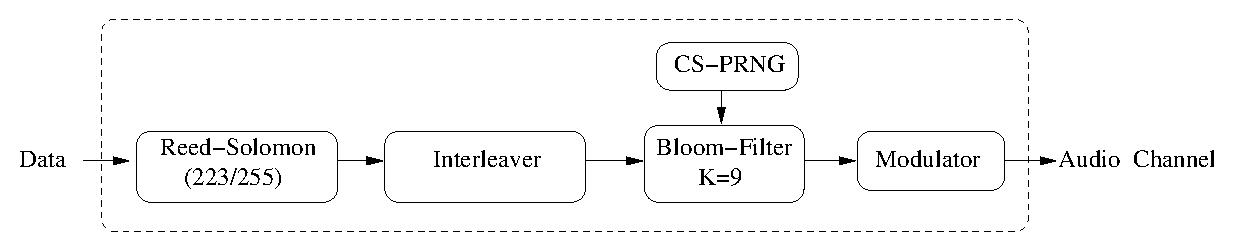
\includegraphics[width=0.9 \textwidth]{Soft-stack2.eps} 
\caption{Etapas del sistema de comunicaciones}
\label{fig_comstack}
\end{figure}

\section{Códigos correctores de errores}

La selección del código corrector de errores debe ser guiada por los parámetros del sistema, sin olvidarse de las posibles limitaciones de calculo del sistema, que es una limitación importante al operar con enlaces con tasas de transmisión elevadas.

En nuestro caso se utilizó un típico arreglo de dos códigos de corrección, uno denominado exterior, encandenado con el segundo denominado interior.
La idea de utilizar dos codigos distintos es la de aprovechar las virtudes de dos tipos de corrección. El código exterior suele ser un código itearativo o convolucional, con una elevada cantidad de paridad y alto poder de detección y corrección. Ciertos tipos de códigos tales como LDPC o codigos Turbo se caracterizan por poseer un piso de error elevado, que es un fenomeno en donde el código pierde efectividad con SNR altos. Esto se soluciona utilizando un segundo codigo corrector denominado interior, que si bien no es tan efectivo a SNR altos como el codigo exterior, es efectivo con SNR bajos, haciendo que el sistema sea efectivo en cualquier condición.

Un parámetro importante en estos algoritmos es el delay, o sea la cantidad de tiempos (medida usualmente en clocks del procesador) que tarda un bit que entra a la etapa de corrección en salir de la misma, luego de la aplicación de la corrección. Este delay es variable segun el algoritmo, algunos algoritmos con un delay importante no pueden ser utilizados en aplicaciones de bajo ancho de banda, ya que retrasan enormemente las comunicaciones. A continuación se detalla el algoritmo de corrección seleccionado.

\subsection{Reed-Solomon}
Como código interior se seleccionó el algoritmo Reed-Solomon, un código de bloque con alta efectividad en SNR bajos. Los parametros seleccionados para dicho código son (255,223) o sea, 223 bytes de datos y 32 bytes de paridad. Estos parámetros lograran que el código pueda detectar hasta 32 errores de byte y corregir hasta 16 errores de byte en los 223 bytes del bloque. La selección de estos parametros responde a que el algoritmo de reed-solomon posee implementaciones muy eficientes si se utiliza un tamaño de bloque de 255 bytes. 
Al ser un estandard muy utilizado, existen implementaciones muy eficientes de reed-solomon con estos parametros especificos, tanto en software como en hardware.
Existen dos problemas con este algoritmo:

1) Elevado delay: Si bien el delay de codificación es mínimo, el delay de decodificacion es muy elevado, pudiendo sobrepasar facilmente los 1200 clocks.
2) Si bien el delay de decodificacion es elevado y requiere mucho procesamiento, el solo echo de tener que acumular un bloque de 256 bytes de datos solo para comenzar con la decodificacion, introduce un retraso muy importante especialmente si el sistema se utiliza con bajo ancho de banda, tal como es el caso en la implementacion acustica del sistema.

Ambos problemas se solucionan seleccionando parametros de Reed-Solomon con un menor tamaño de bloque, o un algoritmo similar con menor tamaño de bloque tal como BCH. El problema en este caso es encontrar implementaciones eficientes de los decodificadores ya que no son algoritmos muy utilizados, por lo que la seleccion final fue el estandard Reed-Solomon (255, 223).

Para la simulación numérica por software se utilizó la biblioteca libfec de Phil Karn~\cite{libfec}. Para la implementacion en FPGA se utilizo la implementacion del algoritmo provista de manera gratuita en la biblioteca de nucleos de IP de Xilinx.

%Con posibilidad de error de simbolo P, la posibilidad de error de un codigo reed-solomon R(n/k) es:
%$$P_{rs}= \sum_{k=(\frac{n-k}{2}+1)}^{n} \binom{L}{i} * P^{i} * (1-P)^{L-i} $$
El código (255,223) es particularmente eficiente de implementar digitalmente ya que cada símbolo puede representarse con un byte (existen 255 símbolos). El código posee 32 bytes de paridad y 223 bytes de datos, lo que representa una adicion de 14\% a la cantidad total de datos a transmitir. Este código permite corregir hasta 16 bytes errados, que pueden estar consecutivos, por lo que RS suele utilizarse en canales con errores de tipo ``Erasure'' o errores tipo ráfaga, donde los errores no estan uniformemente distribuidos sino que estan agrupados temporal o espacialmente.

%En ciertas ona ventaja muy importante es que el codigo de correccion exterior puede facilmente detectar la presencia de un error aunque no pueda corregirlo. Esta informacion es una lista con las posiciones en las cuales se tiene la certeza que los símbolos fueron interferidos denominada lista de síndromes, y puede suministrarse al algoritmo de correccion de errores para que la capacidad de corrección del mismo puede aumentar hasta un 100\%~\cite{Moon:05}.

\subsubsection{Características fisicas}
Un parámetro importante en la selección del algoritmo es la facilidad de implementación sobre hardware digital. Ciertas caracteristicas se vuelven importantes al pasar de implementaciones de software a hardware, tales como tamaño, memoria utilizada y velocidad máxima alcanzada con el hardware disponible, apuntando a que el sistema debe funcionar a tasas de gigabit.

A continuación se nombraran las características de la implementación en hardware (FPGA) de Reed-Solomon utilizada.
El bloque de IP se denomina Reed-Solomon Encoder/Decoder 7.1 de LogiCORE IP. La complejidad espacio-temporal y ciclomática de los algoritmos de codificación de Reed-Solomon son muy distintas a las de su correspondiente algoritmo de decodificación. En general, la decodificación es mucho mas costosa en terminos de recursos de hardware y de latencia agregada al sistema.

Segun la especificacion de esta implementación~\cite{Xilinx:DS252} el decodificador Reed-Solomon con configuracion CCSDS (que implementa el estandard (255,223)) posee un tamaño de 1364 LUTS (Look-up tables) y 3 bloques de RAM. Como comparación, el diseño completa posee un tamaño de aprox. 20000 LUTS, y la FPGA utilizada posee una capacidad de 50000 LUTS y unos 200 bloques de RAM. La velocidad maxima de este algoritmo en la FPGA utilizada es de unos 350 Mhz.
Mucho menor es la cantidad de recursos utilizados por el codificador: Son necesarios solo unos 300 LUTS y solo 1 bloque de memoria aunque la velocidad máxima es similar~\cite{Xilinx:DS251}.

\subsubsection{Cálculo de latencia}
La latencia en un sistema esta dada por el tiempo en que un bit tarda en atravesarlo en su totalidad. Específicamente la latencia de esta estapa es importante ya que la latencia agregada por este algoritmo representa un porcentaje importante de la latencia total de la pila de comunicacion del sistema. Es importante notar que los calculos son específicos de una implementación en particular. 

La latencia total estara dada por la introducida por la codificación adicionada a la de la decodificación ya que los datos deben atravesar ambas etapas. Pero los tiempos de latencia para la codificación son despreciables, en el orden de 5 clocks. 

La latencia de la etapa de decodificación es muy superior y puede ser calculada de manera exacta mediante ecuaciones provistas por la hoja de datos. Una manera simplificada es utilizar la figura \ref{fig_rslat} para obtener el delay de procesamiento. El parámetro $t$ se calcula como $t=(n-k)/2$ donde $n$ es la cantidad de simbolos totales en el bloque (en nuestro caso 255) y $k$ es la cantidad de símbolos de datos en el bloque (223 en nuestro caso) por lo que la variable $t=16$.  El retraso total introducida por la decodificación estara dada por la latencia (en nuestro caso aprox. 650 clocks) mas el retraso producto de cargar un bloque entero de datos en el decodificador, que no es despreciable ya que deben ingresarse los datos al bloque IP por medio de un bus serial de un byte de capacidad, por lo que se necesitan de 255 clocks adicionales por cada bloque. 

Sumando ambos valores e ignorando la mínima latencia de codificación, podemos afirmar que la latencia introducida por el algoritmo Reed-Solomon en el sistema es de 900 clocks.

\begin{figure}[t]
  \centering
  \includegraphics[width=0.6 \textwidth]{graphs/rsDelay.pdf} 
  \caption{Delay de proceso de la implementación de Reed-Solomon utilizada.}
  \label{fig_rslat}
\end{figure}


\subsection{Optimizaciones propuestas}
 
Existen ciertas optimizaciones que podrian haberse realizado si se hubiera optado por reimplementar el algoritmo desde cero, pero que al utilizar una implementacion pre-existente no se realizaron. Estas optimizaciones estan relacionadas con la caracteristicas del canal asimétrico, que presenta las ventajas de tener la certeza de que ciertos símbolos fueron transmitidos correctamente. Una posible optimizacion de Reed-Solomon para su utilización sobre canales Z se plantea para una trabajo futuro.

\section{Canal Z con filtros de bloom}

En esta sección vamos a modelar el canal por el cual estamos transmitiendo datos, específicamente el modelo de ruido del mismo. 
Un canal de comunicaciones puede clasificarse primeramente segun el tipo de información transmitida, sea binaria o analógica, por lo cual tendremos canales binarios o analógicos \cite{MacKay:2002}.
Una sub-clasificación del canal de comunicación puede realizarse segun el comportamiento del ruido del mismo.
Por ejemplo las comunicaciones por radiofrecuencia suelen modelarse como un canal analógico AWGN (Additive White Gaussian Noise). 
El tipo de canal que mejor modela las transmisiones digitales por fibra óptica es el denominado canal Z (Z-Channel), un canal digital en el que el ruido afecta solo uno de los símbolos a transmitir.

Es este modelo de ruido lo que nos permite innovar en el diseño de algoritmos adaptándolos y optimizandolos para aprovechar la naturaleza del error, ya que la mayoria de los algoritmos de corrección de errores estan pensados para un canal de ruido simétrico y generalmente analógico.
Empezaremos primeramente estudiando un modelo simplificado del canal por el cual vamos a trasmitir, el mencionado canal simétrico binario, para despues ahondar en un caso especial de este mismo, denominado Canal Z.

\section{Probabilidad de error de canal binario simétrico}
\begin{figure}[t]
  \begin{center}
    \includegraphics[scale=0.43]{capacidad/canalBinario.png}
  \end{center}
\caption {Canal binario: esquema de probabilidad}
\label{fig:canbin}
\end{figure}

Para calcular el ruido en un canal simétrico binario, calculamos la probabilidad de no-colision que tendra un usuario determinado, ya que las colisiones seran el ruido del canal (En esta etapa no consideramos otros tipos de ruido que pueda tener el canal físico).

\noindent Cantidad de slots por trama: $m$
\noindent Cantidad de usuarios: $n$

\noindent Probabilidad de no colisión para un usuario en un canal simétrico:
\begin{equation}
P_{nc}=\left(\frac{m-1}{m}\right)^{n-1}
\end{equation}


\noindent Probabilidad de no colisión para un usuario en un canal óptico:
\begin{eqnarray}
P_{nc} & = & P(1) \cdot P_{nc}(1) + P(0) \cdot P_{nc}(0) \\
P_{nc} & = & \frac{1}{2} \cdot 1 +  \frac{1}{2} \cdot \sum_{i=0}^{n-1} 
C^{n-1}_{i} \left(\frac{m-1}{m}\right)^i  \left(\frac{1}{m}\right)^{n-1-i}  \left(\frac{1}{2}\right)^{n-1-i} 
\end{eqnarray}

\noindent Donde $\left(\frac{m-1}{m}\right)^i$ es la probabilidad de no
colisión de $i$ canales (se suma para todo posible número de canales no
colisionando: $1\leq i\leq n$, que están en otro slot), $
\left(\frac{1}{m}\right)^{n-1-i}$ es la probilidad de colisión de los restantes
$n-1-i$ (estos están en el mismo slot que el canal actual, el `$-1$' es para no
contar el canal actual), y la colisión se produce cuando los otros canales
transmiten $1$ cuya probabilidad es $\left(\frac{1}{2}\right)^{n-1-i}$. El
factor $C^{n-1}_{i}$ suma sobre todas las combinaciones posibles de canales no
colisionando, que son hechos independientes.

\noindent Teniendo en cuenta que $ \sum_{i=0}^{n-1}
C^{n-1}_{i} \left(\frac{m-1}{m}\right)^i  \left(\frac{1}{2m}\right)^{n-1-i}$ es la potencia $n-1$ de un binomio, reemplanzando tenemos
\begin{eqnarray}
P_{nc} & = & \frac{1}{2} +  \frac{1}{2} \cdot \left(\frac{m-1}{m} + \frac{1}{2m} \right)^{n-1} \\
P_{nc} & = & \frac{1}{2} +  \frac{1}{2} \cdot \left(1- \frac{1}{2m} \right)^{n-1} \\
P_{nc} & \simeq & \frac{1}{2} +  \frac{1}{2} \cdot e^{-1/2} 
\end{eqnarray}

\noindent Donde la última aproximación vale para $n=m$ y $n$ grande.

\iffalse

\vspace{5mm}

\noindent Para el caso de {\em bloom} filters con $k$ filtros\footnote{Se envían $k$ repeticiones del bit en canales distintos, entonces basta que sólo uno de ellos sea 0 para que recibamos un 0 en un canal óptico.} la probabilidad de no colisión es:
\begin{eqnarray} 
P_{nc}^{k} & = &  P(1) \cdot P_{nc}^{k}(1) + P(0) \cdot P_{nc}^{k}(0)\\ \label{Pnc_k}
\end{eqnarray}
Sabiendo que la probabilidad de no colisión para el 0 es:
\begin{eqnarray}
P_{nc}^{k}(0) & = & 1 - \big(P_{c^k}(0)\big)^k 
\end{eqnarray}
Pero la probabilidad de colisión para el 0 cuando se transmiten $k$ copias es:
\begin{eqnarray}
P_{c^k}(0) & = & 1 - \big(P_{nc^k}(0)\big)  \enspace,
\end{eqnarray}
y que además la probabilidad de no colisión para los $k$ slots del bloom
filter es
\begin{eqnarray}
P(\mbox{no col.} k) &=& P(\mbox{no col.}1)\cdot P(\mbox{no col.}2)\cdot P(\mbox{no col.}3)\cdots P(\mbox{no col.}k)\\
&=&\left(\frac{m-1}{m}\right)\cdot\left(\frac{m-2}{m-1}\right)\cdot\left(\frac{m-3}{m-2}\right)\cdots\left(\frac{m-k}{m-(k-1)}\right)\\
&=& \frac{m-k}{m} \enspace.
\end{eqnarray}
Luego la probabilidad de colisión con alguno de las $k$ copias del bit es
\begin{eqnarray}
P(\mbox{col.}k)&=& 1-P(\mbox{no col.} k)\\
&=& 1-\frac{m-k}{m}\\
&=& \frac{k}{m} \enspace.
\end{eqnarray}
Entonces reemplazamos y calculamos:
\begin{eqnarray}
P_{c^k}(0) & = & 1 - \left(\sum_{i=0}^{n-1} C^{n-1}_{i} \left(\frac{m-k}{m}\right)^i \left(\frac{k}{2m}\right)^{n-1-i} \right)  \\
& = &  1-\left( 1-\frac{k}{2m}\right)^{n-1}
\end{eqnarray}
Reemplazando esta ecuación en~\ref{Pnc_k} obtenemos:
\begin{eqnarray}
P_{nc}^k & = & \frac{1}{2} + \frac{1}{2} \left( 1- \left( 1- \left( 1- \frac{k}{2m} \right)^{n-1}  \right)^{k}  \right) 
\end{eqnarray}

Sin embargo, este calculo es incorrecto, comparandolo con los datos que da el simulador. La formula entrega valores de error menores con respecto a los reales, como se observa en la figura. 
Los trazos del mismo color corresponden a el mismo K con azul(K=1), verde (K=2) y rojo(K=4). M=256

\subsection{Entropía}

Comenzemos por lo básico:

Segun Shannon, el \textbf{contenido de informacion} h(x) de un suceso x dada la posibilidad que suceda P(x) es:
$$ h(x) = log_{2}\left(\frac{1}{P(x)}\right) $$

Y la entropia de un conjunto A, H(A) se define simplemente como el promedio del contenido de información:

$$ H(A) = \sum_{x E A_{x}} P(x)log_{2}\left(\frac{1}{P(x)}\right)$$

En un canal binario solo dos sucesos existen, uno con probabilidad p, y otro con probabilidad 1-p, por lo tanto para p siendo la probabilidad de error:

$$ H(p) = -p log_{2}(p)-(1-p)log_{2}(1-p) $$

\subsection{Entropia condicional}

Vamos a analizar la entropia de dos conjuntos X de entrada y Y de salida interrelacionados.

La entropia condicional de X dado $y=b_k$ donde $b_k$ es un valor dado, es la entropia de la distribucion de probabilidad $P(x|y=b_{k})$:
$$H(X|y=b_{k}) = \sum_{x \in A_{x}} P(x | y=b_{k})\log_2\left(\frac{1}{P(x | y=b_{k})}\right) $$

La entropia codicional de X dado Y es el promedio, sobre y, de la entropia condicional de X dado y:
$$H(X|Y) =  \sum_{xy \in A_{x}A_{y}} P(x,y)\log_2\left(\frac{1}{P(x,y)}\right) $$

\subsection{Información mútua}
La información mútua entre X e Y es:
$$I(X;Y) = H(X)-H(X|Y)$$
Mide el promedio de reduccion de la incertidumbre acerca de x que resulta de saber el valor de y, o viceversa: la cantidad promedio de informacion que x revela acerca de y.

\fi
\subsection{Capacidad de canal}

La capacidad C de un canal discreto sin memoria es :

\begin{equation}
C = \max_{{\cal{P}}_x} I(X;Y) 
\end{equation}

O sea, la máxima información mutua entre los alfabetos X de entrada e Y de salida.
Para hallar el máximo podemos derivar $I(X;Y)$ con respecto a la probabilidad $P_x$.
De \cite{MacKay:2002}, para un canal binario asimétrico sin memoria con probabilidad de error $p$, la capacidad máxima $C$ es:

\begin{equation}\label{Cap}
C \approx 1 - H(p) 
\end{equation}

Si expandimos H(p) en \ref{Cap}:

$$ c = 1-\left(p \times \log_2\left(\frac{1}{p}\right) + (1-p) \cdot \log_2\left(\frac{1}{1-p}\right)\right) $$
Simplificada:
$$ c = 1 + p * \log_2(p) + (1 - p) * \log_2(1-p) $$

%Sin embargo esta capacidad es menor que la que realmente tenemos en nuestro canal, ya que un Z-channel se adecua mayormente a los medios de transmisión ópticos. Describiremos en detalle este caso especial en la siguiente sección. ??

\subsection{Canal Z}
Un canal Z (Z-channel) difiere de un canal binario, ya que las probabilidades de bit-flip son asimetricas.
Los Z-channel se usan generalmente para modelar sistemas de transmision opticos.

\begin{figure}[th]
  \begin{center}
    \includegraphics[scale=0.5]{capacidad/zchannel}
  \end{center}
  \caption{Diagrama: Z-channel}
  \label{fig:Gal}
\end{figure}

Para un Z-channel, la distribucion de probabilidades de I(X;Y) es diferente \cite{Tallini:02}, por lo que obtenemos un máximo diferente:

\begin{equation}\label{CapA}
C_{Z} \approx 1 - \left(\frac{1}{2}*H(p)\right)
\end{equation}

Por lo tanto, expandiendo H(p) en \ref{CapA}:

$$ C_{Z} = \log_2\left(1+(1-p) p^{p/(1-p)}\right) $$

La diferencia entre las capacidades de ambos tipos de canal puede apreciarse facilmente en la figura \ref{fig:CompBZ}, donde no tiene sentido hablar de una probabilidad de error mayor a 0.5 en un canal binario simétrico, es totalmente válido en un canal-Z y el mínimo de capacidad en este caso no es cuando $p=0.5$ sino cuando $p=1.0$.

\begin{figure}[th]
  \begin{center}
    \includegraphics[scale=0.9]{capacidad/comparacionBZ}
  \end{center}
  \caption{Diagrama: Azul: Capacidad de canal binario, Verde: Capacidad de canal Z}
  \label{fig:CompBZ}
\end{figure}


\subsection{Filtros de bloom}
Como se discutió en la seccion [TODO], la colisiones de símbolos son inherentes a la modulación seleccionada.
En la modulacion OOK utilizada en un medio óptico, solo los ‘1’s transmitidos pueden interferir con ‘0’s. Este comportamiento puede ser modelado como un canal-Z porque la superposición de pulsos de luz individuales representando ‘1’s puede solamente ser identificados como un ‘1’s, por que la interferencia solamente puede ser aditiva. De esto se desprende que un ‘0’ recibido es un signo inequívoco de la ausencia de pulsos en el slot de tiempo leido.
Una buena estructura para representar este tipo de datos es el filtro de Bloom \cite{Bloom70space/timetrade-offs}, que se utiliza generalmente en técnicas de hashing, utilizándolo para tests muy rápidos (O=1) de pertenencia de un miembro en un set.
La manera en que se implementó este algoritmo en el sistema propuesto se basa es copiar cada bit en K slots del frame transmitido, siendo el frame la representación física del filtro de Bloom. 
En el extremo receptor es suficiente para recibir un solo ‘0’ entre las K copias del bit, para correctamente inferir que el bit original era originalmente un ‘0’, mientras que si el bit original era un ‘1’, las colisiones no tienen efecto debido a la naturaleza del canal-Z.

%As discussed in section 2, this leads to collisions. Since the modulation format is OOK, only transmitted ‘1’s can interfere with ‘0’s.
%This behaviour can be modelled as a Z-channel because the superposition of individual light pulses representing ‘1’s
%can only be identified as a ‘1’, but a received ‘0’ is an unmistakable sign of the absence of pulses in a given time slot.
%We found that the Bloom filter [2] provides a convenient structure to correct for errors in this type of channel. This
%technique is borrowed from hashing algorithms and is used to test whether an element is member of a given set. The
%way that we implement this algorithm relies on copying every bit in K slots of the transmitted frame. On the receiving
%end it is sufficient to receive a single ‘0’ out of K copies in order to correctly retrieve the original transmitted ‘0’,
%whereas collisions have no effect on ‘1’s.

\section{Time-hopping con filtros de bloom}

\section{Minimización de peso de Hamming}
%% extraido de dline-pub.text

Repasando, el esquema propuesto basado en time-hopping CDMA se basa en la interferencia entre símbolos para obtener confidencialidad, ya que los datos de los otros usuarios actuan efectívamente como ruido.
La interferencia inter-símbolo, como fue discutida en la seccion \ref{principle}, causa errores que debe ser corregidos. Como dichos errores reducen el ancho de banda utilizable del canal, es deseable reducir la interferencia hasta un punto donde se maximize, sin comprometer la seguridad del sistema. Para reducir la interferencia, no es aconsejable modificar o introducir patrones en el generador criptograficamente seguro de numeros aleatorios, ya que comprometeria la seguridad de todo el sistema al introducir predictabilidad en las posiciones de los símbolos (Ej. usando códigos ortogonales como en Ref.~\cite{Nadarajah2006}.), efectivamente dejando de ser criptograficamente seguro.
En lugar de esto, se adopto una estrategia que aprovecha el echo que un sistema óptico puede ser modelado como un canal-Z.

%This channel presents a Shannon limit of $ C_{Z} = \log_2\left(1+(1-p) p^{p/(1-p)}\right),$ where $p$ is the probability of error~\cite{Tallini:02}.

Esta propuesta, y aqui esta el nucleo de la invencion propuesta en esta tesis, es la de aprovechar la naturaleza asimetrica del este tipo de canal, en donde solamente el símbolo ``1'' causa interferencia, ya que los ``0'' no se interfieren. \footnote{Aunque en un sistema óptico real, existe efectivamente una pequeña diferencia ya que un ``0'' nunca es representado con una potencia de laser de cero watts.}
En otras palabras, la interferencia de un canal-Z es proporcional al peso de hamming del símbolo transmitido.
El peso de Hamming de un símbolo es simplemente la cantidad de bits en ``1'' del mismo. El algoritmo de Minimización de peso de Hamming consiste en una codificación en donde cada símbolo binario es convertido en un equivalente de mayor longitud, tieniendo solamente una mínima cantidad de dígitos en ``1''. Aplicando esta codificación que minimiza el peso de Hamming y transmitiendo el símbolo resultante, se obtiene una menor interferencia en un canal Z.
Intuitivamente, expandir el símbolo original a uno de mayor longitud decrementaria el ancho de banda del canal; pero como las simulaciones numéricas muestran (ver sección \ref{simulations}) a medida que la interferencia inter-símbolo se reduce, el ancho de banda adicional utilizado por los algoritmos de FEC tambien se reducen, compensando por el incremento del largo del símbolo y logrando un mayor ancho de banda neto del sistema.
Podemos decir que un número binario normal de largo L posee un peso variable de Hamming, con L/2 siendo el promedio, cero siendo el mínimo y L siendo el máximo peso de Hamming.
La técnica de reduccion de peso de Hamming (HW) da buenos resultados reduciendo a HW=2, logrando un buen balance entre la reducción de interferencia y el largo de símbolo.
Adicionalmente, es deseable en un sistema de seguridad que no se revele ninguna información acerca de los símbolos transmitidos. Por ejemplo si transmitieramos el número cero, representado por todos sus dígitos en cero, seria trivial identificarlo sin importar si se aplica cualquier tipo de time-hopping. Para evitar estos ataques que utilizan estadísticas acerca del peso de hamming, la codificación exige que el peso de hamming sea fijo en todos los símbolos. Esto causa una ligera perdida en el ancho de banda pero hace imposible inferir cualquier tipo de información acerca del símbolo transmitido analizando estadisticas de tráfico de los datos transmitidos.

\begin{table}[t]
\begin{center}
\begin{tabular}{c c c}
Datos & entrada HW= 0 to 3 & Expandida HW=2\\
\hline\hline
0 & 000 & 00011\\
1 & 001 & 00110\\
2 & 010 & 00101\\
3 & 011 & 01100\\
4 & 100 & 01010\\
5 & 101 & 01001\\
6 & 110 & 10001\\
7 & 111 & 10010\\
\end{tabular}
\caption{Tambla de minimización de Hamming para símbolos de 3-bits}
\label{hwtable}
\end{center}
 \end{table}
 
\section{Expansión de símbolo}
La minimización del peso de hamming conlleva una necesaria conversión del símbolo original a otro que necesariamente tendra mayor longitud, o sea, una expansión del símbolo.
Esta operación puede realizarse de muchas maneras, pero un algoritmo muy eficiente es utilizar una tabla de lookup (ver tabla~\ref{hwtable}), donde un símbolo de largo L es utilizado como el índice en la tabla, y el resultado es el símbolo expandido, que tiene un largo N\textgreater L.
Por motivos prácticos y de optimización, es deseable que L sea 8 u 16 bits, por lo que la tabla contendrá 256 o 65536 entradas respectivamente.
Al aplicar la minimización de peso de hamming a símbolos de 8 o 16 bits de longitud, son necesarios 256 o 65536 símbolos de salida con un HW=2. En el caso de símbolos de entrada de 8 bits, la longitud del símbolo de salida sera de 363 bits, mientras que para 8 bits de entrada, el simbolo expandido con HW=2 tendra 24 bits de longitud.
Puede observarse que el número de símbolos únicos con HW=2 y N=363 no es exáctamente 65536 sino 65703, esto significa que existen muchas tablas de expansión.
La tabla seleccionada y el orden de la misma no son importantes para el resultado final, observando la condición que dos nodos comunicandose deberan utilizar idénticas tablas.
%In general more bits transmitted per frame the more efficient the protocol will be. \textbf{PORQUE IN GENERAL? CUANDO FALLA?} 


\section{Sistema completo}
%% De orte.tex
El sistema propuesto esta compuesto primeramente de una capa de acceso, donde es implementada la codificación CDMA y corrección de errores, y una capa física basada o bien en una red óptica con similaridades a redes PON, o una red sónica de broadcast.
La capa de acceso es implementada utilizando CDMA del tipo time-hopping, donde cada uno de los $128$ ONUs posibles codifica su información en bits y los envia en un slot seleccionado de manera aleatoria en un frame de $356$ slots\footnote{ Estos valores pueden por supuesto variar de acuerdo a los parametros como error aceptable y cantidad de clientes máxima.}. De esta manera, ocurriran multiples colisiones entre diferentes ONUs pero seran subsanadas por la capa de corrección de errores que garantiza una transmisión de datos virtualmente\footnote{aunque es implosible eliminar totalmente los errores, un BER de 10E-12 se considera libre de errores} libre de errores.

Nota rque la sincronizacion es realizada solo a nivel de bit-slot, en contraste con técnicas como TDMA que deben sincronizar a nivel de frame. También se elimina el requerimiento de una transmisión ordenada en el tiempo; en el esquema propuesto ambos clientes comunicantes pueden empezar su comunicación en cualquier momento, de manera similar al comportamiento del protocolo ethernet.
Un cierto ONU $X$ puede recibir mensajes de otro ONU $Y$ si y solo si $X$ posee la {\em clave} de $Y$, y vice versa. De esta manera, si un cierto grupo de ONUs desean comunicarse sobre VLAN, es requerido que cada una en el grupo conozca todas las otras {\em claves}.

Los flujos de datos de las ONU's se codifican con las siguientes técnicas de corrección de errores (Fig. \ref{arch:chain}):

Reed-Solomon ($223/255$) y algoritmos LDPC ($1024\times512$ matrix) (ver \cite{Moon:05} y sus referencias), ademas de un filtro de Bloom con $K=4$~\cite{Bloom70space/timetrade-offs}.

La seleccion de estos algoritmos de corrección de errores fue influenciada al considerar al canal de comunicaciones como el denominado canal Z, que posee un limite de Shannon de $ C_{Z} = \log_2\left(1+(1-p) p^{p/(1-p)}\right),$ donde $p$ es la posibilidad de recibir un error al transmitir un bit.
Este limite de capacidad es mayor que el límite en una canal simétrico sin memoria \cite{Tallini:02}.

\section{Aplicación en distintos medios físicos}
\subsection{Redes ópticas}
% de orte.text
\begin{figure}[!t]
  \centering
    \includegraphics[width=3in]{orte01.pdf}
    \caption{Proposed network design: Access Layer}
    \label{arch:chain}
\end{figure}
% Fiber		Es grave el efecto de la dispersion?  Sugerimos dispersion shifted G.653? O son muy caras?
% splitter	No 1x128 commercially available (attenuation $\leq 27\,dB$)
% DFB		http://cess-dk.com/gfx/upload/PX2-1541SF.pdf ( min $\simeq-1\,dB$)
% APD		http://pdf.dzsc.net.cn/200810212/286762.pdf ( max $\simeq-27\,dB$)
% EDFA		http://www.lambdaphoto.co.uk/pdfs/EDFADatasheet.pdf

Al adaptar el sistema propuesto a una red óptica, la topología de misma debe ser de tipo estrella (ver Fig.\ref{arch:fig1}) donde splitters ópticos redistribuyen el tráfico proveniente de cada ONY a todo el resto permitiendo comunicaciones punto-a-punto asi como punto-a-multipunto entre hasta $128$ ONUs.
%Traffic redistribution is made by optical splitters at the redistribution hub that introduces high attenuation to optical streams.
Un amplificador óptico de fibra de Erbio (Erbium-Doped Fiber Amplifier, EDFA) localizado entre los splitters en el repetidor óptico incrementa la potencia óptica para contrarrestar las perdidas en la red. 

La modulación utilizada para las señales ópticas es RZ \footnote{La modulacíon RZ o ``Return to Zero'' es la mas común utilizada en fibras ópticas, aunque por razones técnicas en ralidad el laser nunca retorna a cero. Esto tiene consecuencias para el sistema propuesto como se vera mas adelante.} con velocidades previstas de hasta $10$~Gbps por un laser DBF de $2$~dBm de potencia y $1550$~nm de color/frecuencia. Estos parametros permiten una transmisión de hasta $10$~km entre los nodos si se utiliza fibra óptica mono-modo estandard (ITU-T G.652) hacia el repetidor óptico.

En este hub, un spliter de $128\times 1$ maneja el tráfico de todos los ONUs y es luego redistribuido por el correspondiente splitter de $1\times 128$, canalizando el trafico mezclado de cada ONU a travéz de la fibra de bajada, paralela a la fibra de subida.
La atenuacion de los splitters centrales ($\simeq25$~dB cada uno) sumado a la atenuación propia de la fibra óptica y perdidas por inserción ($\simeq2$~dB y $\simeq1$~dB por tramo) contribuyen a las altas pérdidas que este sistema debe compensar ($\simeq28$~dB en ambos canales de subida y bajada).

De utilizarse sin ningun tipo de amplificación, la atenuación que una señal sufriria entre dos ONUs es la suma de la atenuación de ambos tramos, o sea $\simeq56$~dB, que es un valor extremadamente alto fuera del alcance de la tecnología de detección disponible al momento de la escritura de esta tesis.

Sin embargo es posible pasar por etapas de amplificación intermedias para obtener niveles de señal adecuados. Para proveer la amplificación requerida, un EDFA con $\geq27$~dB de ganancia es colocado entre ambos splitters. Este EDFA incrementa la potencia del tráfico a la salida del primer splitter, elevando la potencia de cada '1' de $\simeq-26$~dBm a $1$~dBm a la entrada del segundo splitter, que sera reducida nuevamente por el mismo a un nivel de potencia de $-27$~dBm, que esta dentro de los parametros aceptables de un fotodetector (PD) comercial de alta sensibilidad (Aprox. ($-28$~dBm)).

La potencia máxima de salida del PD no es un parámetro crítico ya que simulaciones [CUALES?] muestran que solamente se produciran colisiones de hasta diez `1' en un slot, y esto con una posibilidad extremadamente baja.

Aún considerando una ganacia de EDFA constante, la potencia de entrada óptica del PD seria menor ($-17$~dBm) que la que son capaces de soportar dispositivos comerciales ($\sim -5$~dBm).
El nivel de bit `0' es dado por la adición de todos los bits `0' transmitidos por todas las $128$~ONUs.
El nivel de decisión del receptor deberia ser capaz de separar entre este estado y aquel de un simple ONU transmitiendo un solo bit en `1'.
De esto se desprende que la potencia de transmisión del bit `0' debe ser la menor posible, o lo que es lo mismo, el radio de extinción del laser DBF debe ser alto.
El radio de extinción (`1'$/$`0' radio de potencia pico) mínimo requerido por el sistema se discute en las simulaciones numéricas a continuación:

% As collisions occur in this scheme minimal powers are such for the case of a single active Tx in a bit slot. In a bit slot with collisions (two or more `1' bits) power increase could be a concern to APD operation
% Optical transmission is performed by a $2$~dBm $1550$ nm DFB-laser generating a
% $10$ Gb/s RZ modulated optical signal, that is transported by up to $10$
% km upstream fiber (ITU-T G.652) to a redistribution hub (see
% Fig.~\ref{arch:fig1}).
\begin{figure}[!t]
  \centering
    \includegraphics[width=3in]{orte02.pdf}
    \caption{Diseño de red propuesto: Capa óptica}
    \label{arch:fig1}
\end{figure}
% Upstream traffic from all ONUs are merged by a $128\times 1$ splitter and then again redistributed by another splitter $1\times 128$ that channels back merged traffic to each ONU through a downstream fiber identical and parallel to the upstream one.
% Splitters' attenuation ($\simeq25$~dB, estimated) contribute, as well as fiber attenuation and insertion losses ($\simeq2$~dB and $\simeq1$~dB per stretch), amount to high total attenuation ($\simeq28$~dB at each upstream and downstream paths).
% In order to make the system workable it is proposed to place a single EDFA optical amplifier ($\geq27$~dB gain) between both splitters.
% This EDFA rises merged traffic power at first splitter output ($\simeq-26$~dBm `1' active Tx) delivering enough power ($1$~dBm, `1' active Tx) at second splitter input to assure power reaching each ONU ($-27$~dBm, `1' active Tx) allows proper reception by a high sensitivity APD ($-28$~dBm).

\subsection{Redes acústicas}
% de newJIS_140512-1.pdf (paper JIS)
\begin{figure}[!t]
  \centering
    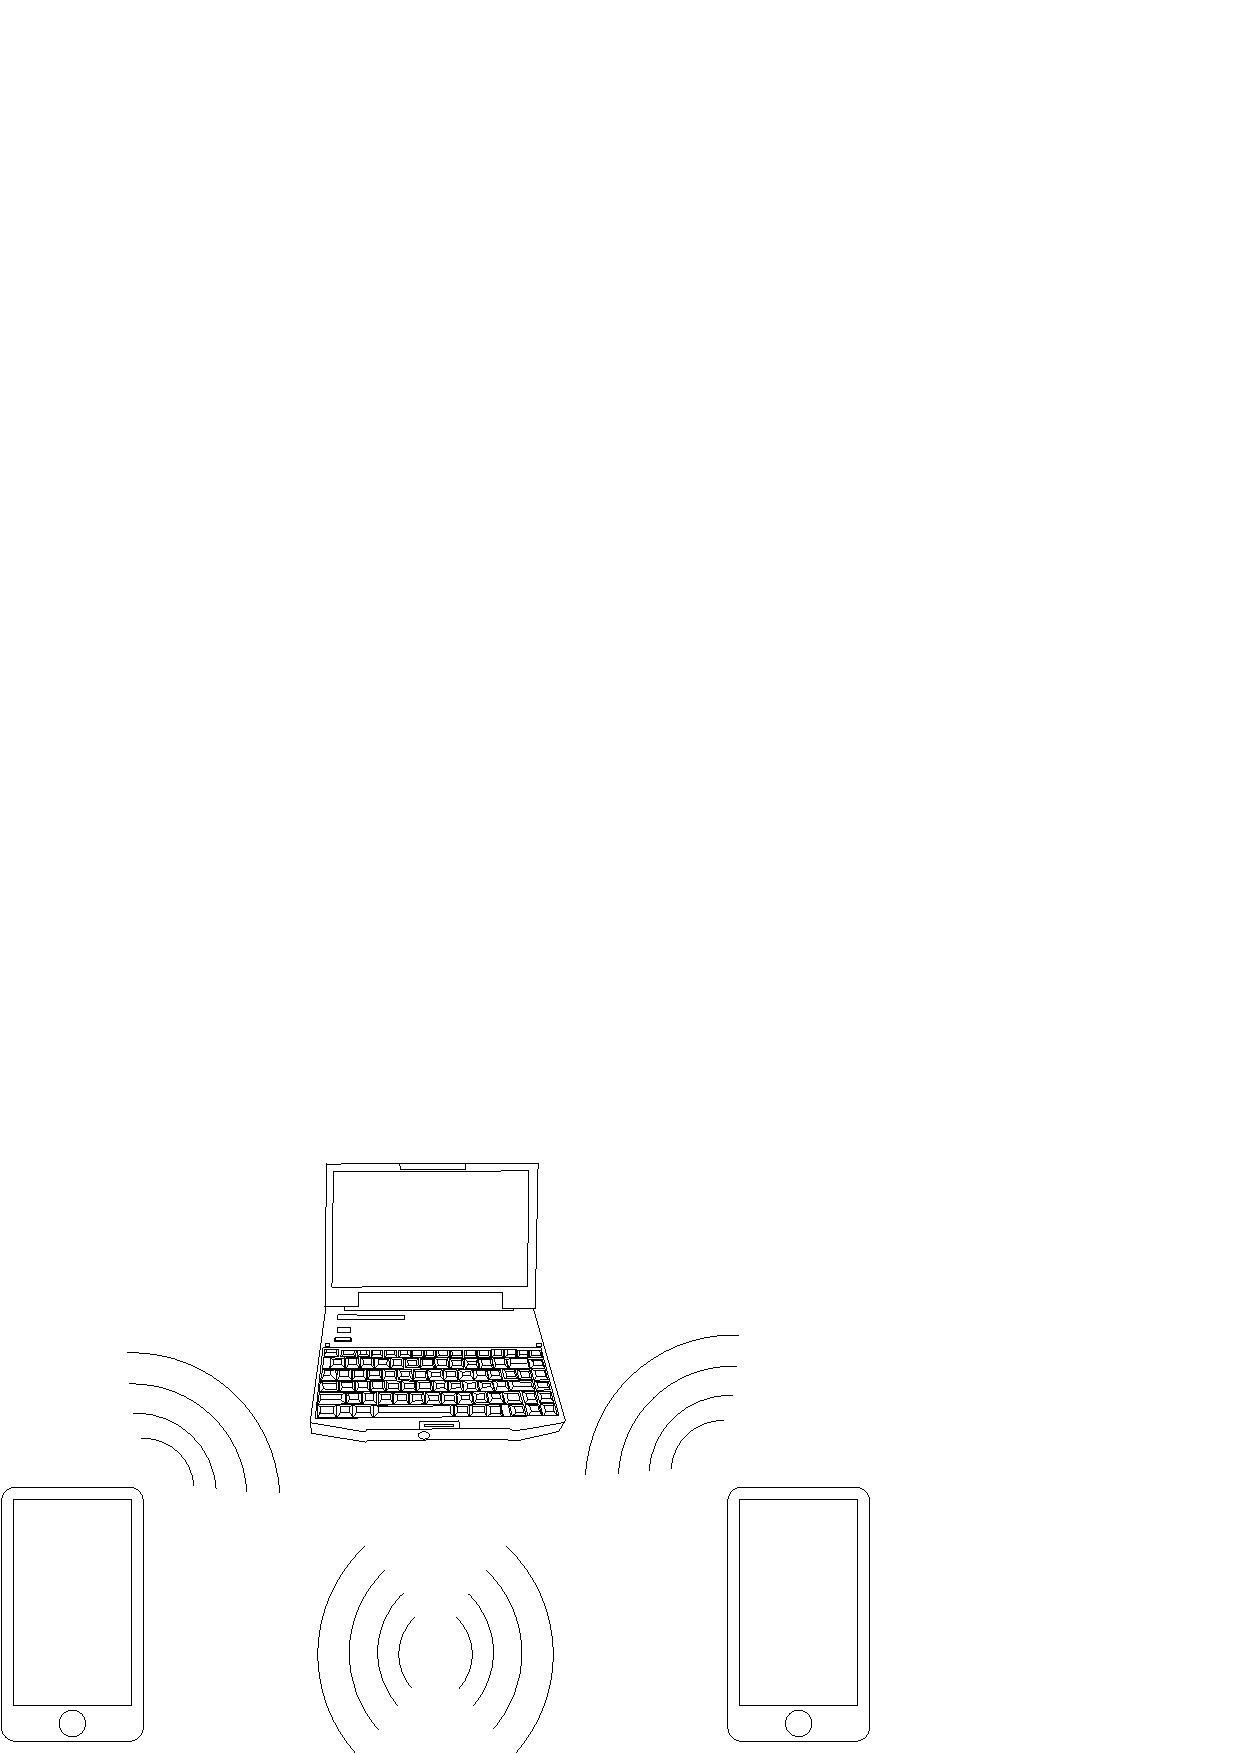
\includegraphics[width=3in]{compucelus.pdf}
    \caption{El diseño de red acústica propuesta puede contener nodos heterogeneos, tales como celulares móviles o computadoras personales.}
    \label{arch:chain}
\end{figure}

Como se discutió anteriormente [DONDE?] es posible utilizar como capa física cualquier canal de comunicaciónes cuyo modelo de ruido o probabilidad de error sea aproximado al de un canal-Z. Un canal óptico es un ejemplo, pero es posible realizar un canal-Z con redes acústicas si se utilizan ciertas modulaciónes y párametros.

Los enlaces ópticos presentan como mayor desventaja la necesidad de, o bien una fibra óptica entre los nodos comunicantes, o que exista visibilidad directa entre ambos nodos, una condición que no puede ser garantizada en muchos ambientes de trabajo. Ademas, los sensores ópticos requeridos generalmente no estan presentes en los clientes y deben ser instalados separadamente.

Sin embargo utilizar un canal acústico tiene como ventaja poder utilizar hardware pre-existente en la mayoria de los potenciales clientes, como parlantes o micrófonos estandard, elementos muy comunes en dispositivos de información actuales [6]. Además, no es necesaria la visibilidad directa mientras ambos nodos esten localizados a pocos cm o metros de distancia, con bajo nivel de volumen.

Pero en contraste con otras tecnologías como RF o enlaces ópticos, la naturaleza del canal de sonido y la facilidad para interceptar o registrar comunicaciones utilizando este medio hace necesaria que la privacidad sea un requerimiento esencial. Muchos sistemas de comunicacion de audio han sido propuestos [7], pero hasta donde fue posible investigar, el problema de la privacidad en este tipo de comunicaciones ha sido solucionada solamente en la capa de aplicación, o sea en alto nivel. Este trabajo presenta una aproximación a la seguridad y privacidad desde la capa física, basada tambien en time-hopping CDMA, similar a aquella presentada en las referencias [8, 9]. En este trabajo se presenta una red segura acústica punto-a-punto y punto-a-multipunto de corto rango y bajo consumo, que no requiere de ningun hardware adicional en clientes moviles.
Establecer un enlace privado entre dispositivos moviles previamente desconectados requiere cierto nivel de interacción por parte del usuario que es usualmente ignorado [5]. Sin embargo, cuando la privacidad se brinda desde la capa física, la intervención del usuario es minimizada. Este es el caso de esta propuesta.

Un escenario válido para la aplicación de esta tecnología podria ser la validación de transacciones financieras pequeñas tales como terminales PoS (Point of Sale) o cajeros automaticos (ATM) utilizando un dispositivo movil (Ej. un smartphone) sin modificaciónes de hardware. Una tecnología similar que se utiliza en estos casos es la denominada Near Field Communications (NFC) [10], un protocolo inalámbrico que requiere hardware especializado que al momento de escritura de esta tesis no se encuentra disponible en la mayoria de los dispositivos moviles.

\subsection{Redes acusticas: Arquitectura}

Una ventaja muy importante del sistema acústico propuesto es su simplicidad, requiriendo solamente un emisor de sonido (parlante), un receptor (micrófono) y un canal de transmisión de sonido que puede ser aire (y en casos mas especializados, agua). Ambos requerimientos estan generalmente disponibles en computadoras, notebooks, tablets y telefonos celulares modernos. 
El esquema lógico es el mismo que el descrito anteriormente: Time-hopping CDMA seguro, códigos correctores de erroes y un método de sincronización a nivel de bit.
Como resultado, el sistema provee canales unidireccionales a los usuarios que sirven tanto para comunicaciones punto-a-punto como punto-a-multipunto. Comunicaciones bi-direccionales pueden establecerse utilizando dos canales separados (Ej. utilizando dos codigos CDMA diferentes), o empleando el mismo canal de manera half-duplex, aunque este último modo de funcionamiento necesita de desarrollo adicional y no es el objetivo de esta tesis.
En las próximas secciones se describe el sistem en mayor detalle.


\chapter{Experiencias realizadas (mediciones)}
\section{Implementación en software}
\subsection{Reed-Solomon}
\subsection{Bloom-filter}
\subsection{Simulador de ruido óptico}
%% de orte.text

El bloque de simulación del canal óptico provee una estimación del BER propio de la fibra óptica del sistema. Los pasos de la simulación son los siguientes:

El tráfico RZ upstream proveniente de todas las ONUs se asume que alcanza al spliter de $128\times1$ con perfecta Sincronización de bit, o sea, sin fluctuaciones (timing jitter).
Los slots correspondientes al bit `0' contienen una pequeña intensidad óptica de CW dada por el razón de extinción de Tx.
Cada ONU on-line en el sistema agrega su propia intensidad de bit `0', incrementando la potencia base total.
Se asume que cada bit `1' agrega un pulso super-Gaussiano ($m=4$) al nivel de potencia base, con un ciclo de trabajo (duty cycle) de $1/3$.


%The physical optical channel simulation block provides an estimate of
%the BER performance of the optical channel. Simulation steps are as
%follows: RZ upstream traffic coming from all ONUs is assumed to arrive
%at the $128\times1$ splitter with perfect time synchronization, i.e., there is no timing jitter. 
%This allows to simulate merged traffic as a simple addition of optical intensities at bit slots for either `0' or `1' bits. % borrar!
%The `0'-bit slots contain a small CW optical intensity given by the Tx extinction ratio. 
%Each on-line ONU adds its `0'-bit optical intensity yielding a base power level.
% As many bit `0' optical intensities are added as on-line ONUs to produce a base power level.  
%Each `1'-bit adds a super-Gaussian ($m=4$) pulse, duty cycle $1/3$, to the base power level. %, with rising edge at slot start and peak amplitude accordingly to Tx optical mean output power.
% As many bit `1' intensities are added to base level as active Tx there are at each simulation bit slot.

Tanto el tráfico saliente como el entrante sufren atenuaciónes debidas a múltiples factores que incluyen pérdidas en el splitter, fibra y empalme (Splice). El presupuesto de potencia (Power budget) se balancea mediante un EDFA con una ganancia constante de $27$~dB. La emisión espontanea amplificada del EDFA es modelada como ruido blanco gaussiano, con una intensidad proporcional a la figura de ruido del amplificador ($7$~dB), y es agregada luego del EDFA.

%Upstream and downstream merged traffic suffers from attenuation due to
%splitter, fiber, and
%splice losses. The power budget is balanced by an EDFA with $27$~dB constant gain.
%Amplified spontaneous emission from the EDFA is modeled by white Gaussian
%noise, with intensity proportional to the amplifier noise figure ($7$~dB), and is added
%after the EDFA. 

%Real EDFAs gain increases with higher input power, i.e. amplification is not
%linear with number of active Txs. Settling for worst case scenario simulation
%we assume same $27\,dB$ gain for any number of active Txs. ASE noise produced
%at EDFA is modelled as a white Gaussian noise added to the optical signal. An
%EDFA accomplishing the amplification previously discussed ($-25.5\,dBm$ to
%$1.5\,dBm$) would have an output SNR $\geq 60\,dB$ accordingly to a estimation
%based on the bandwidth of forthcoming optical filtering at APD detector (see
%section 6.5.1 at~\cite{Agrawal:xx}). Dispersion compensation regeneration stage
%operation is accounted for by simulating no dispersion effects. Traffic is
%routed back to all ONUs by a 1x128 splitter through another $10\,km$
%fiber,
%amounting to a $27.5\,dB$ attenuation; so for one active Tx input power at each
%Rx would be $-27\,dBm$.

La señal de entrada óptica al receptor es filtrada (con un filtro Butterworth de 2do orden y $25$~GHz de ancho de banda) y fotodetectada asumiendo la respuesta de un dispositivo PD estandard (Ver seccion 4.4.3 de ~\cite{Agrawal:xx}).
Posteriormente, ruido blanco gaussiano es agregado, para representar el ruido térmico y ruido de disparo o ruido shot, y un nuevo filtro eléctrico es aplicado (en este caso es un filtro Butterworth de 2do orden y $14$~GHz de ancho de banda). [TODO: Porque?]

%The input optical signal at the receiver is filtered (2nd order low-pass Butterworth filter, $25$~GHz bandwidth) and photodetected assuming a standard PD responsivity (see section 4.4.3 of~\cite{Agrawal:xx}).
%White Gaussian noise accounting for thermal and shot noise is then added
%to the photocurrent, and 
%electrical filtering is applied (2nd order low-pass Butterworth filter, $14$~GHz bandwidth).
%Simulating the decision process a mean of samples around maximum eye opening is compared to a threshold current. 
%Current in case of `1' bits collision is higher than that of a single active Tx, so threshold is established assuming that later case.

%Real EDFAs gain increases with higher input power, i.e., amplification would not be linear with number of active Txs. 
%Settling for worst case scenario simulation we assume same $27\,dB$ gain for any number of active Txs. 
%ASE noise produced at EDFA is modeled as a white Gaussian noise that's added to the electric field. 
%An EDFA accomplishing the amplification previously discussed ($-25.5\,dBm$ to  $1.5\,dBm$) would have an output SNR $\geq 100\,dB$ accordingly to a estimation based on the bandwidth of forthcoming optical filtering at detector (see section 6.5.1 at~\cite{Agrawal:xx}). 
%Effect on traffic of dispersion compensation regeneration stage is accounted by not including in the simulation pulses deformation due to dispersion. 
%Afterwards traffic is routed back to all ONUs by a $1\times128$
%splitter through another $10\,km$ fiber, amounting to a $27.5\,dB$ attenuation arriving to each Rx with $-27\,dB$ for one active Tx.
%
%A concern was if maximum mean total input power allowed at Rx would be surpassed when multiple Tx were simultaneously active. 
%Simulation shown that the occurrence of 15 simultaneously active Tx was a very rare event {\bf <CUANTO??>}. 
%That would amount to $\sim-15\,dBm$ reaching each ONU Rx, well bellow standard commercial Rx overload of $\sim+0.5\,dBm$, that's maximum acceptable mean input power for a BER$<1\,10^{-12}$. 
%
%Rx optical bandwidth is simulated as a low pass filter (2nd order Butterworth as a digital IIR filter~\cite{IIR}, cutoff frequency $25\,GHz$). Afterwards optical traffic is converted into an electrical current. Then to account for thermal and shot noise at a typical APD white Gaussian noise current is added, with an estimated SNR $\simeq 42\,dB$ (see section 4.4.3 at~\cite{Agrawal:xx}). Then electrical filtering is applied (2nd order Butterworth IIR filter, cutoff frequency $6\,GHz$). Detection procedure is performed by comparison to a fixed current threshold. A previous simulation run with the same number of ONUs but with a single active Tx allows to determine the decision threshold at the time of maximum eye diagram opening. Addition of bit `1' amplitudes (collision) produce a current even higher than for a single active Tx, thus this bit slot will be classified as `1' at optical channel simulation output. 
%Media block account for fiber, EDFA and splitters. It attenuates optical trains (splitters and fiber attenuation minus EDFA gain) and also adds white Gaussian noise to the electric field accounting for ASE noise at EDFA. 
% MUCHO, MUY IMPORTANTE: REVISAR CALCULO OSNR (Fn) y verificar que se determina en detector %[VAB]
% ITU recommendation G. 959.1 states that certain interfaces' should operate normally up to $12\,dBm$ mean total input power. In any case if such power is surpassed it would only cause a very short time blinding of Rx affecting a so small amount of bits that wouldn't affect the logical layer ability to correct them.
% receiver overload: max input power for BER<1E-12
%Receiver block simulates Rx behavior. It's optical bandwidth is taken into account by simulating a low pass filtering of incoming traffic (2nd order Butterworth as a digital IIR filter~\cite{IIR}, cutoff frequency $25\,GHz$). Then optical traffic is converted into an electrical current. White Gaussian noise current is added to account for thermal noise at Rx, being it's SNR $\simeq 42\,dB$ accounting for thermal and shot noise at a typical APD detector (see section 4.4.3 at~\cite{Agrawal:xx}). Afterwards another filter simulates detector's linear channel (2nd order Butterworth IIR filter, cutoff frequency $6\,GHz$). Detection procedure is performed by comparison to a fixed current threshold. A previous simulation run with same number of ONUs but with a single active Tx allows to determine the decision threshold at the time of maximum eye diagram opening. Addition of bit `1' amplitudes (collision) produce a current even higher than for a single active Tx, thus this bit slot will be classified as `1' at 
optical channel simulation output. 


%\section{Simulation results}

Las fluctuaciones a niveles de potencia cercanos al límite de sensibilidad del dispositivo PD tienen un importante efecto en la detección de la señal.
El ruido de shot es particularmente preocupante ya que es proporcional al la fotocorriente media. En nuestra propuesta, este ruido es mas alto que en PONs comunes ya que la intensidad del bit `0' de todas las ONUs presentes contribuyen al mismo.
La intensidad resultante de la potencia de base óptica es por lo tanto altamente dependiente del razón de extinción de Tx.
En la Fig.~\ref{sim:optical} se muestra el nivel de razín de extinción mínimo requerido para lograr un BER arbitrario en la capa física como una función del número de ONUs presentes on-line.
%Noise fluctuations at power levels near the PD sensitivity limit have an important effect on signal detection. 
%Detection being made at power levels near PD sensitivity is highly sensitive to changes in noise.
%Shot noise is of particular concern as it is proportional to the mean photocurrent.
%In our network proposal the later is higher than in PONs as bit
%`0' optical intensities from all ONUs are added.
%The resulting base-level optical intensity is then heavily dependent on the Tx extinction ratio.
%Fig.~\ref{sim:optical} shows minimal extinction ratios required to
%achieve an arbitrary BER in the physical layer as a function of the
%number of on-line ONUs.
\begin{figure}[!t]
    \centering
      \includegraphics[angle= 270, width=3.5 in]{orte03.pdf}
%      \caption{Physical layer simulation result: Minimal extinction ratio required to assure a given BER}
      \caption{Resultado de simulaciones de la capa física: Nivel de razón de extinción mínimo requerido para asegurar un cierto BER}
      \label{sim:optical}
\end{figure}
En el escenario de $128$ ONUs presentes, un BER de $<10^{-3}$ puede ser logrado utilizando transmisores del tipo comercial con un razón de extinción de $\simeq16.6$~dB.
Este BER es lo suficientemente bajo para permitir rutinas de corrección de errores al nivel del canal lógico, que garanticen la transmisión libre de errores realizando una utilización acotada de la capacidad total del canal.
%In the $128$ ONUs scenario a  BER$<10^{-3}$ can be achieved using
%commercially available transmitters with an extinction ratio $\simeq16.6$~dB.
%This BER is low enough to allow for logical-channel error-correction routines that guarantee error-free transmission, while still making use of a fair fraction of channel capacity.
% perform correctly and still use a fair fraction of channel capacity.
% Fig.~\ref{sim:optical} shows simulation results for the BER vs OSNR
% for different numbers of ONUs with fixed electrical SNR $\simeq 42$~dB.
% Higher BERs as ONUs number increases due to the higher probability of
% simultaneous bit `1' transmissions (collisions) yielding pulses of
% optical power higher than that of a logical
% `1', generating intersymbol interference. Higher powers generate higher
% currents at Rxs that demand longer times to settle to logical `0' levels after
% filtering. Nevertheless, as
% can be seen in fig.~\ref{sim:optical}, in the worst case scenario (128
% ONUs) the expected OSNR at the EDFA output is enough ($\geq 40$~dB) to
% ensure a BER$<10^{-7}$. In this case simulation shown that the occurrence of
% 15 simultaneously active Tx was a very rare event, so optical power at Rx
% would be $\simeq -15$~dBm, well bellow standard commercial Rx overload
% of $\sim0.5$~dBm (maximum acceptable mean input power for a
% BER$<10^{-12}$).
\begin{figure}[!t]
    \centering
      \includegraphics[angle=270 ,width=3.5 in]{orte04.pdf}
%    \caption{Simulation results: Logical channel}
    \caption{Resultados de la simulación: canal lógico}
      \label{sim:access}
\end{figure}

La Fig.~\ref{sim:access} muestra los resultados de la simulación del canal, comparando el porcentaje logrado con respecto a la capacidad total del canal y el BER medido en un solo canal, con respecto la número de ONUs on-line. Se observan dos mediciones, la primera (círculos) sin incluir el efecto de ruido producido en la capa física, y la segunda (cuadrados) incluyéndolo.
Los resultados fueron obtenidos enviando un gigabit de datos por cada ONU simultáneamente. Esta figura muestra una utilización de canal de $15.7\%$ cuando todos los $128$ ONUs estan transmitiendo simultáneamente, con un BER de $<10^{-8}$. 
De la figura \ref{arch:fig1} podemos observar una penalización de $8$ ONUs cuando el ruido de la capa óptica es tomado en cuenta (Mayormente la razón de extinción y el ruido producido por el EDFA y los PDs).
Considerando que el sistema fue diseñado para soportar comunicaciones asincrónicas (Ej. Ethernet), no es probable que en el uso normal todas las ONUs transmitan simultáneamente; por lo tanto este sistema tiene un BER de $<10^{-8}$ para cada canal cuando 119 ONUs estan transmitiendo al mismo tiempo lo que supone una carga máxima del $90\%$ ($119/128>0.9$). 

%Fig.~\ref{sim:access} shows simulation results for the fraction of the total
%capacity and the BER of one channel at the coding level (circles) and 
%including physical layer impairments (squares). 

%These results were obtained by
%sending one Gigabit of data for each ONU simultaneously.
%This figure shows a channel utilization of $15.7\%$ when all of $128$ ONUs
%are transmitting simultaneously, with a BER$<10^{-8}$. 
%From Fig. \ref{arch:fig1} we observe a penalty of $8$ ONUs when
%impairments from the optical layer (mainly extinction ratio and noise from EDFA and PDs) are taken into account.
%Considering that the system was designed to support asynchronous communications (e.g., Ethernet), it is not likely that all the ONUs will transmit simultaneously (e.g., Internet links often operate at most at $90\%$ load); and therefore our system has a BER $<10^{-8}$ for each channel when 119 ONUs are transmitting at a same time ($119/128>0.9$).
%, removing only one ONU re-establish the desired BER. 
%
%It is worth to remark that, even if the optical channel can induce a
%significant number of errors, the access layer has shown to be able to correct a
%very large number of errors (it is based on
%LDPC+Reed-Solomon+Bloom-Filters), as can be seen on the curve with squares
%at fig.~\ref{sim:access}.
%Observe that the high error rates correspond to a
%worst-case scenario when all ONUs are transmitting simultaneously at
%full capacity, and also 
%there is a low penalty due to physical layer impairments.
%Figure~\ref{sim:optical} presents the simulation's BER vs optical OSNR
%for different numbers of ONUs. %[VAB]
%As the number of ONUs increases higher BERs are obtained at the same optical SNR (electrical SNR is fixed at $\simeq 42\,dB$). In particular there is a penalty of about $30\;dB$ for 128 ONUs in comparison to 1 ONU. This is expected as a consequence of the higher probability of simultaneous bit `1' transmissions (collisions) yielding pulses (logical `1's) of different powers (sum of the power of each transmitter). Higher powers demand more time to settle post filtering current to logical `0' levels. If the following bit slot is indeed a logical `0' an erroneous determination is more possible with a higher collision probability. Nevertheless it can be inferred from simulation results that optical channel should not add significantly to the BER for the whole link as the estimated optical SNR of $\geq 100\,dB$ even for the worst case scenario with 128 ONUs present.
% \begin{figure}[!t]
%     \center
% %     \subfigure[Optical channel]{
% %      \label{sim:optical}
%       \includegraphics[scale=0.4]{BERvsSNR_6GHz.pdf}
% %    }
% %    \subfigure[Logical channel]{
% %      \label{sim:access}
%       \includegraphics[scale=0.4]{BERvsONUs.pdf}
% %    }
%     \caption{Simulation results}
%       \label{archfig}
% \end{figure}

\section{Implementación en FPGA}
El estudio de PONs plantea el desafío de generar, transmitir y recibir
señales de 10 Gbps en el laboratorio. El costo de estos sistemas
suele ser muy elevado. En este trabajo proponemos una alternativa de muy
bajo costo basada en la generación y trasmisión de señales en FPGAs.

\subsection{Arquitectura alto-nivel de la FPGA Xilinx ML507}
El equipamiento consta de un kit de desarrollo ML-507 de Xilinx y un
transceptor SFP+ con láser de 1330 nm, con capacidad de hasta 10 Gbps
en modulación NRZ y alcance de 10km en fibra monomodo. Para realizar
las mediciones presentadas en este trabajo se utilizaron dos dispositivos:
\begin{itemize}
 \item {\em Integrated Bit Error Rate Tester} (iBERT) \cite{4gtxs}: Es
un medidor de tasa de error que utiliza un analizador lógico embebido dentro
del mismo diseño de la FPGA, con interfaz para la herramienta de
verificación y depuración ChipScope. Mediante este agregado, que debe
ser sintetizado dentro del diseño, es posible medir en tiempo real
varios parámetros del transceptor asi como realizar estadísticas y
mediciones de error, variando tasas y características de la transmisión
en tiempo real.
 \item Osciloscopio Óptico Agilent 86100A con módulo óptico 86105A: Para
realizar las mediciones físicas contamos con este equipo que posee un
ancho de banda de 20 Ghz en potencia óptica, suficiente para capturar en
tiempo real los bits individuales o realizar un diagrama de ojo.
\end{itemize}
\subsection{Transmisión a multi-gigabit}
\subsection{Diseño del sistema propuesto}
\section{Redes ópticas}
% de confEUA.tex

\subsection{Transmisión a 9 Gbps con SFP+}
El montaje para la experiencia se realizó conectando el transceptor SFP+
al conector correspondiente en la placa de desarrollo ML-507 y un bucle de
fibra óptica ({\em loopback}), con el objetivo de realizar las
mediciones de BER. Luego, para realizar las mediciones con el
osciloscopio, se debe conectar el extremo de recepción de la fibra
óptica al osciloscopio. En este caso generamos el disparo del
osciloscopio mediante la señal de reloj del sistema (placa ML-507) que
se obtiene a través de los conectores SMA J12 y J13 (si bien es
diferencial sólo utilizamos uno de ellos).  Para la depuración y
configuración se utilizó la interfaz JTAG USB de Xilinx ``Platform Cable
USB II''.
\subsection{Configuración del reloj del transceptor}

La tasa de transmisión del transceptor GTX está dada por la
frecuencia de reloj de entrada $F_{PLL\_Clock}$, donde se transmite un
bit por cada semiciclo (la modulación es NRZ); entonces la tasa de
transmisión será
$R_{line}\mbox{[bps]}=F_{PLL\_Clock}\mbox{[1/s]} \times 2$.  La
frecuencia del reloj de entrada del PLL está gobernada por la ecuación
5-1 \cite[Pag. 88]{ug198}, que reproducimos a continuación:

\begin{equation}
F_{PLL\_Clock} = F_{CLKIN} \times \frac{PLL\_DIVSEL\_FB \times
DIV}{PLL\_DIVSEL\_REF}% \enspace
\end{equation}\\

donde las constantes $PLL\_DIVSEL\_REF = \{1;2\}$, $DIV = \{4;5\} $ y
$PLL\_DIVSEL\_FB = \{1;2;3;4;5\}$ son configurables por software;
mientras que la frecuencia base se configura con las llaves
SW6~\cite[Tabla 1-32]{ug347}: $
F_{CLKIN} (Mhz)= \{62.5;75;77.76;100;125;150;156.25;311.04;622.08\}$.


 Modificando los parámetros puede lograrse, en teoría, un amplio rango
de la frecuencias $F_{PLL\_Clock}$, pero de acuerdo a la documentación
del PLL \cite[Pág. 71]{ug366}~\footnote{La velocidad máxima no se
detalla en la documentación del GTX de Virtex5, pero si en la
documentación del Virtex6, que excepto en el modelo HTX posee parámetros
similares.}, este tiene un rango de operación nominal desde $1.2$ a
$2.7$ Ghz en FPGAs de grado $-1$ tal como el que se encuentra en la
placa de desarrollo ML-507. Sin embargo en este artículo documentamos la
obtención y medición de velocidades de oscilación estables para el PLL
de hasta $4.5$ Ghz (lo que implica una tasa de transmisión de $9$ Gbps),
fuera del rango de operación especificado por el fabricante.

\begin{figure}[t]
  \centering
    %\includegraphics[scale=0.70]{plot.png}
    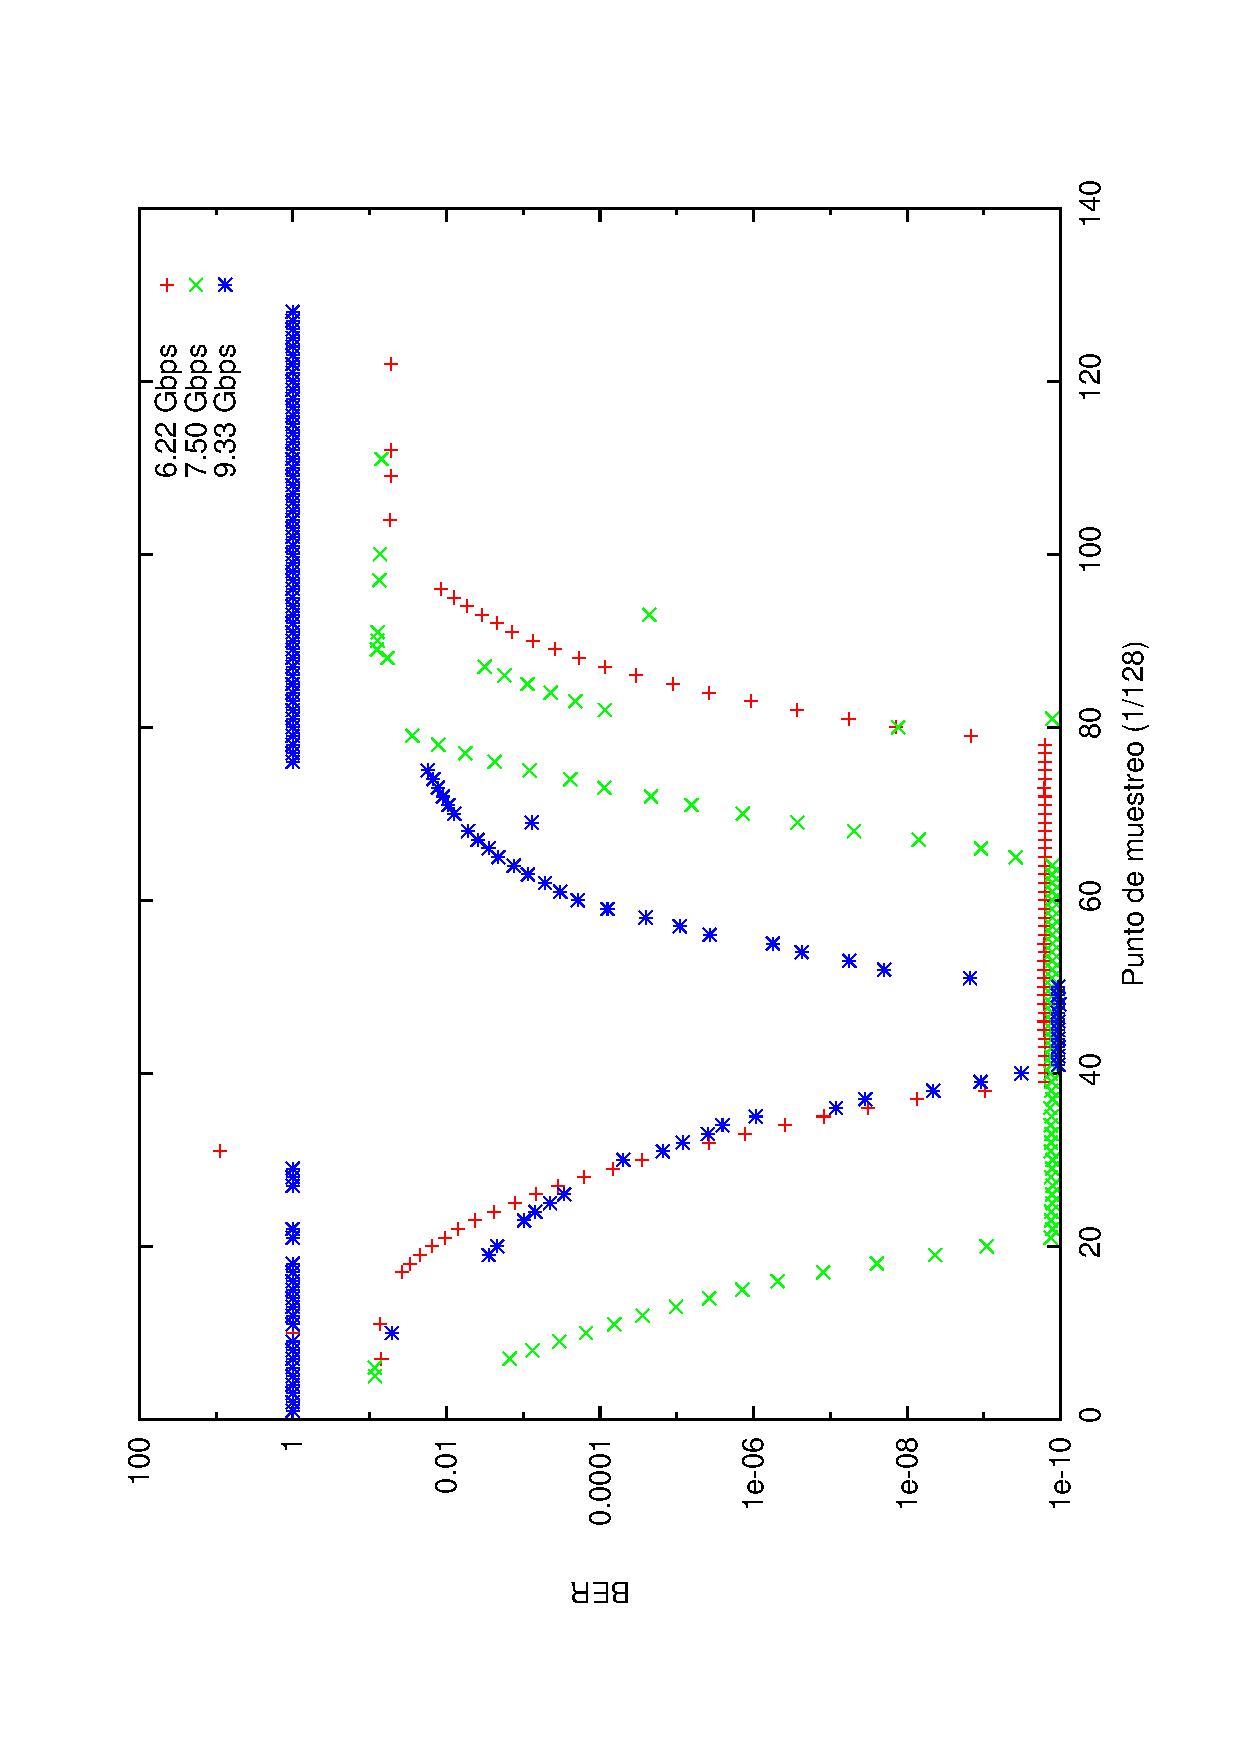
\includegraphics[width=6cm,angle=270]{medicionesPaper/BER_sp.pdf}
\caption {BER vs. punto de muestreo.}
\label{fig:BER}
\end{figure}

\section{Mediciones}
\begin{figure}[!t]
  \centering
%  \subfigure[$4.5$ Gbps]{\includegraphics[scale=0.52]{medicionesPaper/screen3.png}
  \includegraphics[scale=0.52]{medicionesPaper/screen3.png}
  \caption {Señal óptica a $4.5$ Gbps}
  \label{fig:Img1}
%  \\[1cm]
\end{figure}

\begin{figure}[!t]
  \centering
%  \subfigure[$6$ Gbps]{\includegraphics[scale=0.52]{medicionesPaper/screen4.png}
 \includegraphics[scale=0.52]{medicionesPaper/screen4.png}
  \caption {Señal óptica a $6$ Gbps}
  \label{fig:Img2}
%  \\[1cm]
\end{figure}

\begin{figure}[!t]
  \centering
%  \subfigure[$7.5$ Gbps]{\includegraphics[scale=0.52]{medicionesPaper/screen5.png}
 \includegraphics[scale=0.52]{medicionesPaper/screen5.png}
  \caption {Señal óptica a $7.5$ Gbps}
  \label{fig:Img3}
%  }
\end{figure}


\begin{figure}[!t]
  \centering
%  \subfigure[$9.33$ Gbps]{\includegraphics[scale=0.52]{medicionesPaper/screen6.png}
 \includegraphics[scale=0.52]{medicionesPaper/screen6.png}
  \caption {Señal óptica a $9.33$ Gbps}
  \label{fig:Img4}
%  }\\[1cm]
\end{figure}


\begin{figure}[!t]
  \centering
%  \subfigure[$12.44$ Gbps]{\includegraphics[scale=0.52]{medicionesPaper/screen7.png}
 \includegraphics[scale=0.52]{medicionesPaper/screen7.png}
  \caption {Señal óptica a $12.44$ Gbps}
  \label{fig:Img5}
%  }
\end{figure}



\begin{figure}[!t]
  \centering
  \includegraphics[scale=0.52]{medicionesPaper/screen12.png}
  \caption {Señal óptica a $12.44$ Gbps, transmisión 10110101010}
  \label{fig:Img6}
\end{figure}



Las figuras \ref{fig:Img1} a \ref{fig:Img5} muestran la señal óptica producida a diferentes
tasas. Nótese que aunque el equipo puede generar señales estables de
hasta $12.44$ Gbps pero no puede recibirlas a esa frecuencia, por lo que las
mediciones de BER se realizaron solo hasta $9.33$ Gbps. Todas las señales
corresponden a la secuencia 10101010, excepto la figura \ref{fig:Img6},
que fue generada con una secuencia distinta para demostrar el total
control sobre la señal generada. El transceptor posee la capacidad de
realizar una codificación 8B/10B adicional, pero para estas mediciones
ese módulo fue desactivado.



\subsection{Implementación del sistema sobre 8B/10B}
\section{Redes acústicas}

\subsection{Modulación}
% de newJIS_140512
El medio de transmisión sónico utiliza ondas de presión en lugar de electromagnética pero las técnicas de modulación que pueden utilizarse son las mismas.
Sin embargo, no todas las modulaciones siguen el comportamiento de canal Z descrito en la Seccion [TODO].
La modulación On-Off Keying (Un caso especial de modulación ASK, Amplitude Shift Keying), es uno de los tipos de modulación que permite implementar un canal Z sobre un medio acústico si se utiliza sobre cierto rango de parámetros. Utilizando transductores (micrófonos y parlantes) comerciales del tipo presentes en la mayoría de los dispositivos móviles probados, la frecuencia de portadora puede variar de 10 Khz a 16 Khz. Se obtienen resultados buenos con una tasa de transmisión de 1000 bps al nivel de frame. En los experimentos que se detallaran en las secciones siguientes, el retraso (delay) o tiempo que le lleva a un bit atravesar la red, fue extremadamente alto debido a una combinación de baja velocidad de transmisión y la necesidad de un buffer muy grande (1024 bits) necesario para la utilización del esquema de corrección de errores seleccionado (Reed-Solomon 223/255). Si bien aumentar la velocidad de transmisión no es sencillo, modificar el algoritmo de corrección de errores o sus parámetros (Por ejemplo, utilizar algún esquema tipo BCH [12]) podria reducir el delay de datos drásticamente.

Como tecnica de ``pulse-shaping'' se utiliza un simple filtro FIR pasa-banda a la salida de la etapa de modulación, así como también en la entrada de la etapa de demodulación. Este filtro además de reducir el ancho de banda utilizado, ayuda a rechazar interferencias.
Adicionalmente un duty-cycle de 50\% demostró ser el óptimo para la modulación.
%On-Off Keying modulation of sound waves, following the Z-channel interface model described in Section 2.2., encode the transmitted bits as pulses. Carrier frequency can vary from 10 kHz to 16 kHz. Good results can be obtained with a rate of 1000 bps at frame level. In experiments, delay (the time for a bit to traverse the network) was very high, due to Reed-Solomon 223/255 coding, a frame to support up to 16 users and the low capacity of the physical media. A more sensible choice of FEC algorithm (like BCH [12]) could drastically reduce data delay. 

%Simple pulse shaping is realized using a pass-band filter at the output of the modulation and also at the input of the demodulator. This filter also helps reject unwanted interference.
\subsection{Sincronización}
% de newJIS_140512
Como se desprende de la descripción del canal de comunicaciones, la sincronización entre el transmisor y el receptor es esencial para la correcta decodificación de la información. 
En el caso del medio óptico la sincronización de bit y word debe realizarse a tasas tan elevadas que requiere necesariamente soporte de hardware por parte del transceptor.
Sin embargo a las reducidas tasas (1000 bps) utilizadas en el canal acústico permiten realizar una sincronización por software sin ningún soporte de hardware adicional. 
El método es muy similar al utilizado en el canal óptico: Un patrón inicial de sincronización es enviado, para que el receptor pueda realizar un ajuste de parámetros tales como fase y umbral de decisión (Ver Fig. [TODO]). La deriva y fluctuación del reloj del sistema (drift y jitter) no son significantes a esta baja velocidad de transmisión por lo que no se requiere corrección de ningun tipo, haciendo que la Implementación del modem por software sea muy sencilla.
Ciertos parámetros si bien son inicializados en la etapa de sincronización, son por naturaleza dinámicos y se ajustan periódicamente, como por ejemplo el umbral de decisión, que es recalculado a partir de un promedio de los datos de entrada. La fase es también corregida utilizando los datos de entrada como referencia. Notar que este método de sincronización simple permite detectar el comienzo de frame a su vez que se alinea a nivel de bit; ambas alineaciones son necesarias en cada comunicación (pero la alineación de frame solamente entre los ONUs comunicantes). Adicionalmente, una vez comenzada la transmisión, los datos seran indecifrables gracias al algoritmo de time-hopping guiado por un CS-PRNG.

%As it follows from the description of the communication channel, synchronization between the transmitter and receiver is essential for the correct decoding of information. For this purpose, an initial synchronization pattern is sent, so the receiver can adjust parameters like phase and decision level (see Figure 3). For the data bits transmission a duty cycle of 50\% showed in our experiments an enhanced detection. Clock drift and jitter are not significant at this low transmission speed and so no correction is required, making the software modem implementation very simple. Decision level is dynamic, meaning it is constantly re-calculated from averaged input data. The receiver symbol phase is also corrected using the input data as reference. Notice that this simple synchronization method allows detecting the frame start as well as the bit slot; both are needed at every communication. Moreover, once the data began to be transmitted, the communication becomes indecipherable thanks to the CS-PRNG.



\subsection{Medición multi-usuario}
\subsection{Medición distintas distancias}

\section{Conclusiones}

\chapter{Conclusiones}
En este capítulo final se presenta un resumen, conclusiones y futuros trabajos que se desprenden de esta tesis.

\section{Resumen o Sumario}

Se presentó un sistema de comunicaciones privado del tipo broadcast capaz de crear múltiples VLANs utilizando cualquier medio de transmisión que pueda ser modelado como un canal-Z.
Para ello, fue necesario desarrollar varios algoritmos y codificaciones con el objetivo de proveer principalmente privacidad.

Se demostró la viabilidad del proyecto mediante implementaciones de prototipos tanto sobre fibra óptica con velocidades de transmisión de 5 Gbps implementados sobre una FPGA, y con un segundo prototipos puramente implementados por software, que utiliza el mismo protocolo, esta vez sobre una red encriptada acústica entre dispositivos móviles sin ningun tipo de modificación.

\section{Conclusiones}

\section{Trabajo futuro}



% ********************************************************************
% Backmatter
%*******************************************************
\appendix
\cleardoublepage
%\part{Apéndice}
%\include{Chapters/Chapter0A}



% ------------------------------------------------------------------------

%BIBLIOGRAFIA
\linespread{1.44}
%\bibliographystyle{amsplain}
\bibliographystyle{ieeetr}
%\bibliographystyle{alpha}
\bibliography{vb_fgct,IEEEabrv,IEEEorte,confEUA,misc}

% =================================================================
% Dummy directive
% Included for Gather Purpose only:
% %input "Xbib.bib"
% is no longer necessary because
%  \bibliography{xbib}
% is now defined as an input directive
% (see Options -> Advanced -> Tree [INPUT_DIRECTIVES] for details...
% It can be reconfigured!
% =================================================================
\end{document}
% ------------------------------------------------------------------------
